\documentclass[12pt,oneside]{memoir}
\usepackage{multirow}
\usepackage{matfmaster}
\usepackage{anyfontsize}

% Opcija [b5paper]:
%   ako želite da napravite verziju teze u manjem (b5) formatu, navedite
%   opciju "b5paper", tj. prethodni paket uključite pomoću: 
%   \usepackage[b5paper]{matfmaster}. Tada ima smisla razmisliti o promeni
%   veličine slova (izmenom opcije 12pt na 11pt u \documentclass{memoir}).
%
% Naravno, opcije je moguće kombinovati.
% Npr. \usepackage[b5paper,biblatex]{matfmaster}

% Paket koji obezbeđuje ispravni prikaz ćiriličkih italik slova kada
% se koristi pdflatex. Zakomentarisati ako na sistemu koji koristite ovaj
% paket nije dostupan ili ako ne radi ispravno.
\usepackage{cmsrb}
\usepackage{xcolor}
% Ostali paketi koji se koriste u dokumentu
\usepackage{listings} % listing programskog koda

\lstdefinestyle{mystyle}{
    keywordstyle=\color{orange},
    basicstyle=\ttfamily\footnotesize,
    breakatwhitespace=false,         
    breaklines=true,                 
    captionpos=b,                    
    keepspaces=true,                 
    numbers=left,                    
    numbersep=5pt,                  
    showspaces=false,                
    showstringspaces=false,
    showtabs=false,                  
    tabsize=2
}
\lstset{style=mystyle}

% Datoteka sa literaturom u BibTex tj. BibLaTeX/Biber formatu
\bib{matfmaster-primer}

% Ime kandidata na srpskom jeziku (u odabranom pismu)
\autor{Зорана Гајић}
% Naslov teze na srpskom jeziku (u odabranom pismu)
\naslov{Савремене библиотеке за прикупљање података са веб-страница}
% Godina u kojoj je teza predana komisiji
\godina{2023}
% Ime i afilijacija mentora (u odabranom pismu)
\mentor{др Милена \textsc{Вујошевић Јаничић}, ванредни професор\\ Универзитет у Београду, Математички факултет}
% Ime i afilijacija prvog člana komisije (u odabranom pismu)
\komisijaA{др Весна \textsc{Маринковић}, доцент\\ Универзитет у Београду, Математички факултет}
% Ime i afilijacija drugog člana komisije (u odabranom pismu)
\komisijaB{др Александар \textsc{Картељ}, доцент\\ Универзитет у Београду, Математички факултет}
% Ime i afilijacija trećeg člana komisije (opciono)
% \komisijaC{}
% Ime i afilijacija četvrtog člana komisije (opciono)
% \komisijaD{}
% Datum odbrane (obrisati ili iskomentarisati narednu liniju ako datum odbrane nije poznat)
\datumodbrane{Септембар 2023.}

% Apstrakt na srpskom jeziku (u odabranom pismu)
\apstr{%
Прикупљање података са веб-страница има кључну улогу у многим областима истраживања и пословања. За ефикасно прикупљање и парсирање података, неопходно је разумети савремене библиотеке и технике. Овај рад има за циљ да сагледа савремене библиотеке и технике за ефикасно прикупљање и парсирање података са веб-странице и да истакне њихове предности и недостатке, фокусирајући се на њихову имплементацију и функционалности.
}

% Ključne reči na srpskom jeziku (u odabranom pismu)
\kljucnereci{прикупљање података са веб-страница, веб-скрејпинг, парсирање \textit{HTML} кода, библиотека \textit{BeautifulSoap}, библиотека \textit{Selenium}, библиотека \textit{Scrapy}, алат \textit{SPLASH}}

\begin{document}
% ==============================================================================
% Uvodni deo teze
\frontmatter
% ==============================================================================
% Naslovna strana
\naslovna
% Strana sa podacima o mentoru i članovima komisije
\komisija
% Strana sa posvetom (u odabranom pismu)
\posveta{Велика захвалност менторки на саветима и мотивацији и породици на подршци.}
% Strana sa podacima o disertaciji na srpskom jeziku
\apstrakt

% Sadržaj teze
\tableofcontents*

% ==============================================================================
% Glavni deo teze
\mainmatter
% ==============================================================================

% ------------------------------------------------------------------------------
\chapter{Увод}
У данашњем дигиталном добу, велика количина података се налази на интернету, а веб-странице су богат извор информација за многе области истраживања и пословања. Међутим, прикупљање података са веб-страница може бити изазовно због различитих фактора као што су динамичност веб-страница, идентификација елемената у оквиру \textit{HTML} кода и заштита података.

Аутоматизација процеса прикупљања података са веб-страница игра\\кључну улогу у откривању и праћењу трендова, анализи конкуренције, истраживању тржишта, предвиђању потрошачких преференција и многим другим областима. Уместо ручног прегледања и бележења података са великог броја веб-страница, аутоматизација омогућава брзо и ефикасно прикупљање података у великим количинама. Ово не само да штеди време и ресурсе, већ такође смањује могућност грешака и обезбеђује доследност у процесу прикупљања података.

Приступи и алати за прикупљање података са веб-страница су разноврсни и прилагођени специфичним потребама корисника. Постоје библиотеке и софтверски алати који омогућавају аутоматско претраживање веб-страница, екстракцију података и њихово складиштење у жељеном формату. Ови алати често користе технике попут веб-скрејпинга, анализе \textit{HTML} структуре и употребе регуларних израза како би идентификовали и издвојили релевантне податке. Примери библиотека које омогућавају аутоматизацију процеса
прикупљања података су: \textit{BeautifulSoup} \cite{beautifulSoapDocs}, \textit{Selenium} 
 \cite{selenium} и \textit{Scrapy} \cite{scrapy}.

\textit{BeautifulSoup} је Пајтон библиотека која се користи за парсирање \textit{HTML} и \textit{XML} документа. Омогућава једноставно извлачење података из \textit{HTML} страница. Библиотека \textit{BeautifulSoup} пружа моћне функционалности за претраживање и манипулацију \textit{HTML} структурама, олакшавајући проналажење, извлачење и обраду жељених података.

\textit{Selenium} је популарна библиотека за аутоматизацију Веб-прегледача. Омогућава програмско управљање Веб-прегледачем за симулирање корисничких
интеракција са веб-страницом. Ово се доминантно користи у контексту аутоматизације тестирања веб-апликација. Библиотека \textit{Selenium} омогућава програмерима и тест инжењерима да аутоматски интерагују са Веб-прегледачима, симулирају корисничке акције и проверавају очекиване резултате. Аутоматизација тестирања помоћу библиотеке \textit{Selenium} омогућава ефикасно откривање грешака, смањује време и ресурсе потребне за ручно тестирање, као и обезбеђује доследност у извршавању тестова. Поред аутоматизације у тестирању, библиотека \textit{Selenium} се користи и за прикупљање података јер омогућава прикупљање података који се динамички генеришу или су доступни само након одређених корисничких акција, као што су кликови на дугмад или попуњавање формулара.

\textit{Scrapy} је моћна библиотека за прикупљање података са веб-страница. Помаже у претраживању, извлачењу и складиштењу података на структуриран начин. \textit{Scrapy} омогућава брзо и ефикасно прикупљање велике количине података са веб-страница. 

У глави \ref{chp:prikupljanje} су детаљно разматрани изазови са којима је могуће се сусрести приликом прикупљања података са веб-страница, као и процес идентификовања елемената у \textit{HTML} коду. У глави \ref{chp:alati} је дат детаљан преглед наведених библиотека и алата који се користе за прикупљање података. Глава \ref{chp:poredjenje} је фокусирана на поређење наведених библиотека, док је у глави \ref{chp:zakljucak} изложен закључак на основу представљених информација.

% ------------------------------------------------------------------------------
\chapter{Прикупљање података са веб-страница}
\label{chp:prikupljanje}
Веб\footnote{Светска мрежа, познатија као Веб, систем је међусобно повезаних, хипертекстуалних докумената који се налазе на интернету.} (енг. \textit{World Wide Web, WWW}) представља највећи извор података у историји човечанства, али се већина ових података састоји од неструктурираних информација, што може отежати њихово прикупљање \cite{osmarPaper}. 
На многим веб-сајтовима забрањено је копирање и преузимање података, али на сајтовима на којима је преузимање података дозвољено, ручно копирање може потрајати данима или недељама.

Веб скрејпинг (енг. \textit{Web scraping}) представља аутоматизовани процес који омогућава издвајање података са различитих веб-страница и њихово чување у структурираном формату ради тренутне употребе или касније анализе. Постоје различити програмски језици који пружају подршку за имплементацију Веб скрејпинга, од којих су најпопуларнији: Пајтон (енг. \textit{Python}), Јава (енг. \textit{Java}) и Руби (енг. \textit{Ruby}).

Поступак прикупљања информација састоји се од неколико фаза, које су приказане на слици  \ref{fig:web-scraping-steps}. Прва фаза је проналажење одговарајуће веб-странице за прикупљање података (детаљније објашњено у одељку \ref{chp:izazovi}) и одређивање информација које су потребне за прикупљање. Након тога, потребно је послати \textit{HTTP}\footnote{\textit{HTTP} је мрежни протокол који припада слоју апликације референтног модела ОСИ, представља главни и најчешћи метод преноса информација на Вебу.} (енг. \textit{Hypertext Transfer Protocol}) захтев на жељену веб-страницу и преузети изворни кôд \textit{HTML} странице. Пре него што се парсира \textit{HTML} кôд, потребно је пронаћи најбољи начин за индексирање жељених елемената, а затим парсирати изворни кôд \textit{HTML} странице и извршити неопходну радњу са добијеним информацијама \cite{EvalTools}.

\begin{figure}[!ht]
  \centering
  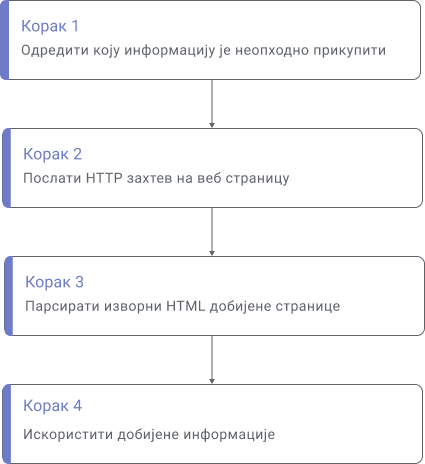
\includegraphics[width=0.5\textwidth]{Zorana Gajic - master rad/slike/veb-skrejping-koraci.png}
  \caption{Фазе прикупљања и употребе података}
  \label{fig:web-scraping-steps}
\end{figure}

\section{Изазови у процесу прикупљања података}
\label{chp:izazovi}

Веб скрејпинг се сматра корисним процесом за добијање увида у податке. Међутим потребно је пазити на правне аспекте, како би се избегли легални проблеми. Важно је напоменути поштовање фајла \textit{robots.txt} који представља политику веб-сајта. Овај фајл може садржати одредбе које забрањују приступ и прикупљање података са одређених делова веб-страница. 
Правилно разумевање закона о ауторским правима, заштити података и других релевантних прописа је од суштинске важности како би се осигурало законито и етичко прикупљање података. Најчешће се фајл \textit{robots.txt} проналази на нивоу основног директоријума. Уколико фајл садржи линије попут ових приказаних у наставку, то значи да веб-сајт не жели да се прикупљају подаци са њега:
\begin{verbatim}
User-agent: *
Disallow:/ 
\end{verbatim}

Да би прикупљање података било успешно, од суштинског значаја је квалитет добијених података.  Како би се добили квалитетни подаци, потребно је да је сам веб-сајт исправан, односно да не садржи неисправне линкове, јер се веб скрејпинг обично изводи преко целог веб-сајта, а не само преко одређених страница.

Када се ради о пројектима великих размера и обимних база података, један од честих изазова јесте складиштење података. Овај изазов је повезан са ефикасним прикупљањем, обрадом и анализом велике количине података који се могу прикупити путем веб скрејпинга са различитих извора. Овај проблем може бити решен употребом већ постојећих платформи за складиштење.

У наставку ће бити описане најчешће заштите од напада на веб-странице који представљају изазове за процес веб скрејпинга:
\begin{enumerate}
\item \textit{CAPTCHA} (енгл. \textit{Completely Automated Public Turing test to tell\\Computers and Humans Apart}).

    \textit{CAPTCHA} је технологија која се користи за проверу и потврду да је корисник веб-странице заиста човек, а не програм \cite{captcha}. Провера се постиже приказивањем изазова, на пример слике са текстом или бројевима које је потребно препознати. Изазов је обично лак људима за решавање, али је тежак за програме који то треба брзо и аутоматски да реше. Корисници обично морају да унесу решење изазова како би потврдили да су људи и како би им био дозвољен приступ подацима на веб-страницама.
\item Захтеви за аутентификацију.

    Пријава корисника на веб-страницу може да представља велики изазов приликом веб-скрејпинга динамичних веб-страница. Уобичајени процес пријаве обухвата уношење корисничког имена и лозинке у одговарајућа поља на веб-страници, а затим клик на дугме за пријављивање. Приликом аутоматизације овог процеса могу се јавити потешкоће, али се оне могу решити уз помоћ библиотека као што су \textit{Selenium} \cite{selenium} и \textit{Scrapy} \cite{scrapy}.

\item Блокирање \textit{IP} (енгл. \textit{Internet Protocol address}) адреса.

    Веб-странице могу блокирати \textit{IP} адресе које се повезују са прекомерним бројем захтева или са ботовима који су идентификовани као нежељени. Ово може бити привремено или трајно.
\item Провера корисничког агента.

    Сваки \textit{HTTP} захтев у заглављу шаље корисничког агента (енг. \textit{user agent}). Коришћењем овог подешавања веб-сајт идентификује претраживач који му приступа: његову верзију и платформу. Уколико се користи исти кориснички агент у сваком захтеву, веб-сајт може лако да открије да је у питању аутоматизовани приступ страници.
\item Праћење учесталости прикупљања података.

    Како би се избегло преузимање садржаја са веб-странице у превеликој количини или превеликој брзини, веб-сајтови могу имплементирати ограничења фреквенције за ботове. Ова ограничења имају за циљ да контролишу број захтева по јединици времена и максималну брзину преузимања.
    
    Важно је разумети да ова ограничења нису постављена да би се спречило легитимно прикупљање података, већ да би се заштитио веб-сајт од претераног оптерећења. Уколико веб-сајт има велики обим података или има ограничене ресурсе, ограничења фреквенције су неопходна како би се осигурала стабилност и доступност сајта за све кориснике.
\end{enumerate}

\section{Идентификација елемената у оквиру \textit{HTML} кода}
Веб скрејпинг технологије подразумевају различите методе и библиотеке за издвајање података са веб-страница. У оквиру ових технологија користе се: регуларни изрази (енг. \textit{Regular Expressions, RegEx}), тагови (енг. \textit{tags}), \textit{CSS} (енг. \textit{Cascading Style Sheets}) селектори и \textit{XPath} \cite{xpath} (енг. \textit{XML Path Language}).

Препоручени редослед идентификације елемената у оквиру \textit{HTML} кода током веб скрејпинга је следећи:

\begin{enumerate}
\item Преко идентификатора --- ако елементи имају јединствени идентификатор, најбрже и најпоузданије је користити овај начин идентификације.
\item По имену класе --- ако се елементи налазе у истој класи, могу се идентификовати преко имена класе. Ово је корисно када је потребно издвојити групу елемената са заједничким стилом или функционалношћу.
\item По таговима --- ако је неопходно издвојити све елементе са одређеним тагом, овај начин идентификације је најбољи.
\item \textit{CSS} селектори --- ако постоје елементи који немају јединствен идентификатор, али имају јединствен \textit{CSS} стил, могу се идентификовати преко \textit{CSS} селектора.
\item Регуларни изрази --- ако је неопходно издвојити елементе на основу текста који се налази у њима.
\item \textit{XPath} --- ово је најопштији начин идентификације елемената у \textit{HTML} коду.
\end{enumerate}

\subsection{Идентификатори и имена класа}
Када елементи на веб-страници имају јединствен идентификатор, најбржи и најпоузданији начин иденфитикације је коришћење тог идентификатора. Идентификатор је обично атрибут \texttt{id} у \textit{HTML} коду и служи као јединствено име за одређени елемент. Користећи идентификатор, могуће је директно циљати жељени елемент без потребе за додатним филтрирањем или селекцијом.

Ако се елементи на веб-страници налазе у истој класи, могуће је идентификовати их на основу имена класе. Класа је атрибут \texttt{class} у \textit{HTML} коду и користи се за груписање елемената са сличним стилом или функционалношћу. Коришћење имена класе омогућава издвајање групе елемената са заједничким карактеристикама. Ово је корисно када је неопходно издвојити више елемената одједном.

Када користимо идентификаторе или имена класа за издвајање елемената са веб-страница, важно је разумети да ови идентификатори или класе нису универзални и да се могу разликовати између различитих сајтова. За сваки сајт је потребно проучити структуру \textit{HTML} кода и идентификовати одговарајуће идентификаторе или класе које је неопходно издвојити.

Одређивање тачних идентификатора или класа за сваки сајт може бити процес који захтева проучавање \textit{HTML} структуре, инспекцију елемената и анализу \textit{CSS}-а. Ово је специфично за сваки појединачни сајт и не постоји универзална аутоматска метода за проналажење свих потребних идентификатора или класа.

Како бисте одредили које идентификаторе или класе треба користити, треба да се користе следеће методе:
\begin{itemize}
\item Проучавање \textit{HTML} кода и идентификација атрибута \texttt{id} и \texttt{class}  који се користе за циљане елементе.
\item Анализа \textit{CSS}-а како бисте идентификовали стилове или селекторе који су повезани са жељеним елементима.
\item Употреба инспектора веб-прегледача који омогућава преглед и интерактивно истраживање \textit{HTML} структуре и стилова.
\end{itemize}

Важно је напоменути да је приступ издвајању података путем идентификатора или имена класа осетљив на промене у структури или дизајну веб-страница. Ако се структура \textit{HTML} кода или стилови сајта промене, идентификатори или класе које смо користили можда више неће бити тачни. Стога је важно редовно проверавати исправност и ажурирати кôд за издвајање података уколико се страница мења.

\subsection{Тагови}
Тагови играју кључну улогу у прикупљању података са веб-страница јер помажу у идентификацији и издвајању одређених информација из изворног кода \textit{HTML} страница. Тагови у \textit{HTML} коду се користе за дефинисање структуре веб-странице. Сваки таг представља одређени елемент или секцију странице, као што су заглавља, пасуси, слике и линкови.

У наставку су наведени тагови који се најчешће користе:
\begin{itemize}
    \item \texttt{<html>} --- Oзначава почетак и крај HTML документа.
    \item \texttt{<body>} --- Представља садржај документа који је видљив кориснику.
    \item \texttt{<h1>} до \texttt{<h6>} --- Користе се за дефинисање наслова.
    \item \texttt{<p>} --- Користи се за дефинисање параграфа текста.
    \item \texttt{<a>} --- Ствара хиперлинк (енгл. \textit{hyperlink}) до друге веб-странице.
    \item \texttt{<ul>} и \texttt{<li>} --- Користе се за стварање неуређене листе ставки.
    \item \texttt{<ol>} и \texttt{<li>} --- Користе се за стварање уређене листе ставки.
    \item \texttt{<div>} --- Користи се за дефинисање одељка документа у сврху стилизовања.
    \item \texttt{<span>} --- Користи се за дефинисање малог дела текста у сврху стилизовања.
\end{itemize}

\subsection{\textit{CSS} селектори}
\textit{CSS} селектори се могу користити у процесу сакупљања података са веб-страница како би се идентификовали и издвојили одређени елементи. Овакав приступ је посебно користан када се ради са веб-страницама које не поседују јасну структуру и организацију. 

\textit{CSS} селектори раде на принципу идентификације елемената према њиховом имену ознаке, имену класе или идентификатору. На пример, селектор  \texttt{div[class='imeKlase']} се користи за издвајање свих \textit{div} елемената који имају класу \textit{imeKlase}.

\subsection{Регуларни изрази}
Регуларни изрази представљају метод за усклађивање специфичних образаца у зависности од датих комбинација, који се могу користити као филтери за добијање жељеног резултата. У прикупљању података регуларни изрази се често користе за поређење шаблона и издвајање података, за локализовање и издвајање специфичних података из \textit{HTML} или \textit{XML} докумената. Једна од најзначајнијих предности регуларних израза јесте у њиховој универзалности, тј. могу се применити на било коју врсту података. 

У многим програмским језицима, регуларни изрази се подржавају кроз уграђене библиотеке или модуле. Модул \textit{re} програмског језика Пајтон пружа подршку регуларним изразима за поређење шаблона и издвајање података.

У наставку је дат пример регуларног израза који се може користити за претраживање и издвајање свих веб-адреса из изворног кода \textit{HTML} странице. 
Конкретно, тражи се почетак хипервезе \textit{a} која садржи атрибут \textit{href}, а затим се издваја веб-адреса из овог атрибута и ставља у групу. У овом примеру регуларни израз користи знакове за постављање групе, односно за издвајање дела шаблона. Унутар овог израза, веб-адреса се ставља у групу помоћу парова заграда.
\begin{lstlisting}[language=Python]
regex_pattern = r"<a\s+(?:[^>]*?\s+)?href=\"([^\"]*)\""
\end{lstlisting}

\subsection{Језик \textit{XPath}}
Језик \textit{XPath} представља флексибилан начин адресирања различитих делова
\textit{XML\footnote{\textit{XML} представља прошириви (мета) језик за означавање (енгл. \textit{markup})}} (енг. \textit{Extensible Markup Language}) документа који су у формату \textit{XML} или неком сличном формату. То га чини погодним за навигацију кроз објектни модел било ког таквог документа\footnote{Објектни модел документа представља хијерархијски приказ структуре веб-сајта.} (енг. \textit{Document Object Model, DOM}), уз помоћ језика \textit{XPath} (енг. \textit{XPathExpression}). Израз у језику \textit{XPath} дефинише образац за одабир скупа чворова и садржи преко 200 уграђених функција \cite{xpath}. Овај језик је дефинисао \textit{WWW} конзорцијум. У овом раду ће се језик \textit{XPath} користити за одабир елемената са изворног кода \textit{HTML} страница.

\subsubsection{Синтакса језика \textit{XPath}}
Језик \textit{XPath} користи изразе путања за избор чворова у \textit{XML} документу. Чвор се одабира праћењем путање или корака. 

Неки корисни примери израза путања су наведени у наставку:
\begin{description}
\item \texttt{//h2} --- Издваја све елементе \textit{h2}.
\item \texttt{//div//p} --- Издваја све елементе \textit{p} који се налазе унутар блока \textit{div}.
\item \texttt{//ul/li/a} --- Издваја све линкове који се налазе унутар неуређених листи.
\item \texttt{//ol/li[2]} --- Издваја други елемент уређене листе.
\item \texttt{//div/*} --- Издваја све неурђене елементе који се налазе унутар блокова \textit{div}.
\item \texttt{//*[@id=''id'']} --- Издваја елемент са идентификатором \textit{id}.
\item \texttt{//*[@class=''class'']} --- Издваја све елементе са класом \textit{class}.
\item \texttt{//a[@name or @href]} --- Издваја све линкове који имају атрибут \textit{name}, атрибут \textit{href} или оба.
\item \texttt{//a[last()]} --- Издваја последњи линк.
\item \texttt{//table[count(tr)=1]} --- Издваја табеле које имају само један ред у њима.
\item \texttt{//*} --- Издваја све елементе.
\item \texttt{//a/text()} --- Издваја текст линка.
\item \texttt{./a} --- Тачка издваја тренутни чвор.
\end{description}

Неки корисни примери функција у оквиру израза путања су наведени у наставку:
\begin{description}
\item \texttt{string(n)} --- Конвертује друге типове података у ниску. На пример, уколико је \textit{n} број 42, онда ће резултат бити ниска "42".
\item \texttt{number(n)} --- Конвертује друге типове података у број. На пример, уколико је \textit{n} ниска "42", онда ће резултат бити број 42.
\item \texttt{contains(a, b)} --- Проверава да ли се одређена ниска појављује унутар друге ниске. Први аргумент је ниска у којем се врши претрага, а други аргумент је ниска која се тражи. На пример, уколико је \textit{a} ниска "abcdefg", а \textit{b} ниска "bcd", онда ће резултат бити вредност \textit{true}.
\item \texttt{starts-with(a, b)} --- Проверава да ли одређена ниска почиње задатом подниском, односно да ли ниска \textit{a} почиње са ниском \textit{b}.
На пример, уколико је \textit{a} ниска "abcdefg", а \textit{b} ниска "abc", онда ће резултат бити вредност \textit{true}.
\item \texttt{ends-with(a, b)} --- Проверава да ли одређена ниска завршава задатом подниском, односно да ли се ниска \textit{a} завршава са ниском \textit{b}.
На пример, уколико је \textit{a} ниска "abcdefg", а \textit{b} ниска "efg", онда ће резултат бити вредност \textit{true}.
\end{description}
% ------------------------------------------------------------------------------
\chapter{Преглед библиотека за прикупљање података са веб-страница}
\label{chp:alati}
% ------------------------------------------------------------------------------
У оквиру рада биће извршено детаљно прикупљање података са веб-странице \textit{\href{https://www.audible.com/search}{https://www.audible.com/search}}. На главној страници \textit{Audible} веб-сајта налази се бочна секција са списком категорија књига. Свака категорија представља одређену тематску групу књига, као што су "Уметност и забава", "Биографије и мемоари", "Посао и каријера" итд. Унутар сваке категорије, постоји списак књига које припадају тој теми. Да би се приступило свим књигама у једној категорији, потребно је прећи кроз све странице кроз пагинацију. Пагинација омогућава прелазак на следећу или претходну страницу, како би се приказале све доступне књиге у тој категорији. Проласком кроз све категорије и њиховим пагинацијама, могуће је прикупити информације о свим доступним књигама на  веб-страници \textit{Audible}.

\section{Библиотека \textit{BeautifulSoap}}
\label{chp:beaufiulSoap}
Библиотека \textit{BeautifulSoap} \cite{beautifulSoapDocs} је Пајтон библиотека која се користи за парсирање и претраживање \textit{HTML} и \textit{XML} докумената. Ова библиотека подржава различите врсте навигације кроз \textit{HTML} и \textit{XML} документе, као што су претраживање по имену тагова, претраживање по садржају тагова, претраживање по атрибутима тагова и слично.
Једна од главних особина библиотеке \textit{BeautifulSoap} је да је компатибилна са различитим парсерима, укључујући \textit{html.parser} \cite{htmlParser}, \textit{lxml} \cite{lxmlParser} и \textit{html5lib} \cite{html5lib}. За разлику од других библиотека које ће се касније разматрати, ова библиотека не може сама да приступи веб-страници и потребни су јој помоћни модули. 

Библиотека \textit{BeautifulSoap} има многе карактеристике које олакшавају њену употребу. Библиотека се лако инсталира помоћу наредбе \textit{pip} и има једноставан интерфејс (енг. \textit{interface}).

\subsection{Инсталација}
Библиотека \textit{BeautifulSoap} се може инсталирати користећи алат за инсталирање библиотека за програмски језик Пајтон звани \textit{pip} \cite{pip}. Неопходно је покренути следећу наредбу из командне линије:
\begin{verbatim}
pip3 install bs4
\end{verbatim}
Ова наредба ће преузети и инсталирати најновију верзију библиотеке \\ \textit{BeautifulSoap}. Након успешне инсталације, неопходно је увести библиотеку у Пајтон кôд користећи следећу наредбу:
\begin{verbatim}
from bs4 import BeautifulSoup
\end{verbatim}

\subsection{Провера динамичности веб-странице}
Многе веб-странице, укључујући веб-страницу \\ \textit{\href{https://www.audible.com/search}{{https://www.audible.com/search}}}, која се анализира у овом раду, користе динамичке технологије које омогућавају промену садржаја без освежавања целе странице, што представља изазов при парсирању таквих страница. У овом контексту, библиотека \textit{BeautifulSoap} се најчешће користи за анализу \textit{HTML} или \textit{XML} кода веб-страница, али због динамичности неких страница, могуће је да се не ухвате све промене на страници. Због тога се користе библиотеке попут \textit{Selenium} \cite{selenium} и \textit{Scrapy} \cite{scrapy} за праћење промена у реалном времену.

\subsection{Прикупљање \textit{HTML} кода веб-странице}
Библиотека \textit{BeautifulSoup} не представља самосталну библиотеку за прикупљање података са веб-страница. Да би се преузео \textit{HTML} кôд веб-странице неопходно је инсталирати библиотеку \textit{Requests-HTML} \cite{requestsDocs}, која омогућава креирање \textit{HTTP} захтева на одређену веб-страницу и за одговор добија \textit{HTML} кôд те странице. 

Постоји неколико метода од значаја у библиотеци \textit{Requests-HTML} \cite{WebScrapingWithPython}:
\begin{itemize}
    \item \begin{verbatim}get(url, params=None, **kwargs) \end{verbatim}
    Ова метода шаље \textit{HTTP GET}\footnote{\textit{HTTP GET} захтев је метод комуникације у \textit{HTTP} протоколу који се користи за захтевање ресурса са сервера.} захтев на наведену веб-адресу. 
  \item \begin{verbatim}post(url, data=None, json=None, **kwargs)\end{verbatim}
    Ова метода шаље \textit{HTTP POST}\footnote{\textit{HTTP POST} захтев је метод комуникације у \textit{HTTP} протоколу који се користи за слање података серверу ради креирања или ажурирања ресурса.} захтев на наведену веб-адресу. 
  \item \begin{verbatim}put(url, data=None, **kwargs)\end{verbatim}
    Ова метода шаље \textit{HTTP PUT}\footnote{\textit{HTTP PUT} захтев је метод комуникације у \textit{HTTP} протоколу који се користи за ажурирање постојећег ресурса на серверу.} захтев на наведену веб-адресу. 
\end{itemize}
Додатни параметри \textit{kwargs}\footnote{\textit{kwargs} је скраћеница за ”\textit{keyword arguments}” и представља специјални елемент у програмском језику Пајтон који омогућава преношење произвољног број названих аргумената у функцији.} омогућавају спецификацију додатних опција.
 
Неколико уобичајених опционалних параметара из више наведених метода у оквиру библиотеке \textit{Requests-HTML}:
\begin{itemize}
    \item \begin{verbatim}params\end{verbatim} 
        Опциони параметар \textit{params} се користи за слање додатних параметара у \textit{URL} у облику упитних параметара приликом слања \textit{HTTP GET} захтева. Упитни параметри се додају на крај \textit{URL}-а након знака "?" и обично се састоје од имена параметра и његове вредности раздвојених знаком "=". На пример, параметар може да се искористи за филтрирање резултата, сортирање или специфицирање странице у случају пагинације. 
    \item \begin{verbatim}data\end{verbatim} 
        Опциони параметер \textit{data} се користи за слање података у телу захтева приликом слања \textit{HTTP POST} или \textit{HTTP PUT} захтева. Подаци могу бити у облику ниске или у облику речника који ће бити аутоматски кодиран у одговарајући формат.
    \item \begin{verbatim}json\end{verbatim} 
        Опциони параметер \textit{json} се такође користи за слање података у телу захтева приликом слања \textit{HTTP POST} или \textit{HTTP PUT} захтева, али уместо обичне ниске, подаци се шаљу као \textit{JSON} објекат. Библиотека  \textit{Requests-HTML} ће аутоматски серијализовати \textit{JSON} објекат и поставити одговарајуће заглавље захтева.
    \item \begin{verbatim}headers\end{verbatim} 
        Опциони параметер \textit{headers} се користи за специфицирање додатних заглавља \textit{HTTP} захтева. Могуће је користити овај параметар за постављање специфичних заглавља као што су кориснички агент или слање ауторизационог токена.
    \item \begin{verbatim}timeout\end{verbatim} 
        Опциони параметер \textit{timeout} се користи за постављање временског ограничења за чекање на одговор сервера.
\end{itemize}

Кôд приказан на листингу \ref{lst:get-html} представља кôд у програмском језику Пајтон који преузима \textit{HTML} кôд веб-странице. Важно је знати да преузимањем веб-странице помоћу Пајтон библиотеке \textit{Requests-HTML}, постоји могућност да се деси да страница није доступна на серверу (или да је дошло до грешке у њеном преузимању), или да сервер није доступан.
\begin{lstlisting}[language=Python, caption={Прикупљање \textit{HTML} кода веб-странице}, label={lst:get-html}]
import requests

url = 'https://www.audible.com/search'
try: 
    response = requests.get(url) 
except requests.exceptions.RequestException:
    print("Error fetching page")
    exit()    
    
html = response.text
\end{lstlisting}

\subsection{Парсирање \textit{HTML} кода веб-странице}
Пајтон нуди разне библиотеке за парсирање \textit{HTML} кода, од којих су две најзаступљеније: \textit{lxml} и \textit{html.parser}. Парсер \textit{lxml} је најбржи парсер веб-страница према званичној документацији библиотеке \textit{BeautifulSoup} \cite{beautifulSoapDocs}, који може да анализира велике и сложене документе. Парсер \textit{html.parser} је уграђени Пајтон парсер који је намењен да ради са мањим и једноставнијим \textit{HTML} документима \cite{WebScrapingWithPython}.

Да би се извршило парсирање добијеног \textit{HTML} кода веб-странице, прво је неопходно креирати објекат \textit{BeautifulSoup} уз помоћ добијеног \textit{HTML} кода и жељеног парсера. Осим наведеног корака, у Пајтон коду на листингу \ref{lst:parse-html} је приказано да резултат креирања објекта \textit{BeautifulSoup} нуди издвајање наслова и текста веб-странице, поред разних других информација.

\begin{lstlisting}[language=Python, caption={Креирање објекта \textit{BeautifulSoup}}, label={lst:parse-html}]
from bs4 import BeautifulSoup
...
# html objekat je dobijen kao povratna vrednost funckije get modula requests
...
soup = BeautifulSoup(html, 'lxml')
print(soup.text)
print(soup.title.text)
\end{lstlisting}

Добијени објекат \textit{BeautifulSoup} такође омогућава приступ различитим деловима \textit{HTML} кода користећи методе као што су \texttt{find()} i \texttt{find\_all()}. Метода \texttt{find()} користи се када је потребно пронаћи први елемент у \textit{HTML} коду који одговара одређеном тагу или класи. Ова метода враћа први пронађени елемент који одговара постављеним критеријумима, док се метода \texttt{find\_all()} користи када је потребно пронаћи све елементе у \textit{HTML} коду који одговарају одређеном тагу или класи. Ова метода враћа листу свих пронађених елемената који одговарају постављеним критеријумима.

Кôд приказан на листингу \ref{lst:parse-html-books} прикупља податаке о књигама са веб-странице \textit{Audible}. Прво је неопходно преузети \textit{HTML} садржај веб-странице (кôд приказан на листингу \ref{lst:get-html}), а затим креирати објекат \textit{BeautifulSoup} за парсирање  \textit{HTML} садржаја (кôд приказан на листингу \ref{lst:parse-html}). Затим се проналази елемент \textit{div} са класом \textit{"adbl-impression-container"}, унутар којег се проналазе сви елементи \textit{li} са класом \textit{"productListItem"}. За сваку књигу у листи, извлачи се наслов, аутор, датум издања и цена, који се затим додају у одговарајуће листе.

\begin{lstlisting}[language=Python, caption={
Издвајање наслова, аутора, датума издања и цене књиге из \textit{HTML} кода веб-странице}, label={lst:parse-html-books}]
...
# soup objekat je dobijen kao povratna vrednost prilikom kreiranja objekta tipa BeautifulSoup
...
container = soup.find('div', class_='adbl-impression-container')
book_list = container.find_all('li', class_='productListItem')

for book in book_list:
    book_titles.append(book.find('h3', class_='bc-heading').text.strip())
    book_authors.append(book.find('li', class_='authorLabel').a.text.strip())
    book_release_dates.append(substr_after_colon(book.find('li', class_='releaseDateLabel').text.strip()))
    book_prices.append(extract_regular_price(book.find('div', class_='adblBuyBoxPrice').text.strip()))
\end{lstlisting}

\subsection{Прикупљање података са више веб-страница} 
Када се користи библиотека \textit{BeautifulSoup} за прикупљање података са више веб-страница, могу се јавити проблеми у вези са аутоматским прикупљањем података са свих жељених страница. Када се прикупљају подаци са једне странице, обично се користи функција \texttt{get} модула \textit{requests} (листинг \ref{lst:get-html}) за дохват \textit{HTML} кода и затим се креира објекат \texttt{BeautifulSoup} (листинг \ref{lst:parse-html}) за анализу \textit{HTML} кода и издвајање неопходних података. Међутим, ако се подаци прикупљају са више страница, неопходно је итерирати кроз све странице и аутоматски дохватити \textit{HTML} кôд за сваку страницу. На пример, ако странице имају адресе које се разликују само по броју странице, може да се искористи петља која пролази кроз све адресе и дохвата \textit{HTML} кôд сваке странице.

Прилагођавање овог процеса је за сваки веб-сајт специфично. Сваки веб-сајт може имати различиту структуру \textit{HTML} кода и различите \textit{URL} адресе. Аутоматизација овог процеса може бити изводљива у неким случајевима, на пример, ако постоји доследан шаблон \textit{URL} адреса или правилност у структури \textit{HTML} кода. Међутим, често је потребно прилагодити кôд за сваки веб-сајт како би се успешно прикупили подаци. Осим коришћења петље и генерисање \textit{URL} адреса, постоје и друге честе опције које се могу користити за прикупљање података са више веб-страница. Једна опција је употреба интерфејса за програмирање апликација, скраћено \textit{API\footnote{\textit{API} представља скуп правила, протокола и инструкција које омогућавају комуникацију између различитих софтверских компоненти.}} (енг. \textit{Application Programming Interface}) уколико је доступан. \textit{API} омогућава програмски приступ подацима са веб-странице, што може бити ефикасан начин за прикупљање жељених података. Такође треба размотрити коришћење других библиотека као што су \textit{Selenium} и \textit{Scrapy} које пружају напредне могућности за прикупљање података.

На пример, да би се прикупиле све информације о књигама са веб-странице \textit{Audible}, потребно је проћи кроз све категорије и пагинацију на свакој од тих категорија. Коришћењем методе \texttt{find} библиотеке \textit{BeautifulSoup}, проналази се елемент \textit{div} који садржи листу елемената \textit{li}, који представљају веб-адресе за сваку од категорија. Затим је потребно итерирати кроз листу веб-адреса, учитати \textit{HTML} кôд за сваку веб-адресу и пронаћи пагинациони елемент из којег се извлачи број последње странице. Након тога, пролази се кроз све странице одабране категорије. Са сваке странице је могуће извући информације о насловима, ауторима, датумима издања и ценама књига. 

Важно је напоменути да библиотека \textit{BeautifulSoup} не симулира интеракцију са Веб-прегледачем, што означава да итерирање кроз категорије и кроз странице се врши преласком са једне веб-адресе на другу веб-адресу уочавањем обрасца у веб-адреси. Другим речима, за пагинацију је уочено да се вредност параметра \textit{page} мења између 
\textit{page=1}, \textit{page=2}, \textit{page=3} и слично.
\begin{lstlisting}[language=Python, caption={Прикупљање података са више веб-страница}, label={lst:beautiful-soap-scrape-mutliple}]
...
# soup objekat je dobijen kao povratna vrednost prilikom kreiranja objekta tipa BeautifulSoup
...
pagination = soup.find('ul', class_='pagingElements')
pages = pagination.find_all('li', class_='bc-list-item')
last_page = pages[-2].text

for page in range(1, int(last_page) + 1):
    ...
    # html objekat je dobijen kao povratna vrednost funckije get modula requests 
    ...
    html = audible_shared.fetch_html(f'{website}?page={page}')
    soup = BeautifulSoup(html, 'lxml')
    container = soup.find('div', class_='adbl-impression-container')
    titles, authors, release_dates, prices = audible_shared.collect_books_info(container)
    book_titles.extend(titles)
    book_authors.extend(authors)
    book_release_dates.extend(release_dates)
    book_prices.extend(prices)
\end{lstlisting}

\section{Библиотека \textit{Selenium}}
\label{chp:selenium}
Библиотека \textit{Selenium} је популарна библиотека програмског језика Пајтон која се користи за ефикасну аутоматизацију интеракције са веб-страницама. Она омогућава симулирање корисничке интеракције са веб-страницама, као што су уношење текста, кликтање, претраживање елемената и прикупљање података. 

Библиотека \textit{Selenium} пружа богат скуп функција за претрагу елемената на веб-страници, као што су проналажење елемената по идентификатору, имену, класи, ознаци или \textit{XPath} изразу. Ово омогућава једноставну манипулацију одређеним деловима веб-страница. Још једна корисна особина ове библиотеке је могућност руковања чекањима и интеракцијом са динамичким елементима странице. На пример, могуће је да се сачека да се одређени елемент учита пре него што се изврше следеће наредбе.

\subsection{Инсталација}
Библиотека \textit{Selenium}, слично библиотеци \textit{BeautifulSoup}, се може инсталирати користећи алат \textit{pip}. Неопходно је покренути следећу наредбу из командне линије:
\begin{verbatim}
pip3 install selenium
\end{verbatim}
Након успешне инсталације, неопходно је увести библиотеку у Пајтон кôд користећи следећу наредбу:
\begin{verbatim}
import selenium
\end{verbatim}

\subsection{Улога драјвера}
Управљачки програм или драјвер (енг. \textit{driver}) је програм који омогућава комуникацију између програма вишег нивоа, као што је апликација, и физичких компоненти рачунара, као што су тастатура, миш, графичка картица и слично. Када се користи библиотека \textit{Selenium}, није могуће директно комуницирати са Веб-прегледачем (енг. \textit{web browser}), већ је неопходно користити драјвер који ће посредовати у комуникацији између кода и Веб-прегледача и омогућити контролу над Веб-прегледачем користећи библиотеку \textit{Selenium}. За сваки Веб-прегледач постоји одређени драјвер који се користи са библиотеком \textit{Selenium}. На пример, за Веб-прегледач Гугл кроум (енг. \textit{Google Chrome}) се користи драјвер \textit{ChromeDriver}, док се за Веб-прегледач Мозила фајерфокс (енг. \textit{Mozilla Firefox}) користи драјвер \textit{GeckoDriver}.

Како би се омогућило коришћење драјвера у Пајтон коду, потребно је да се преузме одговарајућа верзија драјвера за неопходни Веб-прегледач. Након тога треба навести путању до драјвера и инстанцирати драјвер коришћењем модула \textit{webdriver} из библиотеке \textit{Selenium}. Наведени кôд на листингу \ref{lst:selenium-driver-init} представља претходно описане кораке за случај када је коришћен Веб-прегледач Гугл кроум. Након тога, кôд може да отвори веб-адресу и управља истом. На крају, линија \texttt{driver.quit()} затвара Веб-прегледач и ослобађа коришћене ресурсе.

\begin{lstlisting}[language=Python, caption={Прикупљање \textit{HTML} кода веб-странице помоћу библиотеке \textit{Selenium}}, label={lst:selenium-driver-init}]
from selenium.webdriver.chrome.service import Service
from selenium import webdriver

path = '/usr/local/bin/chromedriver_mac64_arm64/chromedriver'
service = Service(executable_path=path)
driver = webdriver.Chrome(service=service)
website = 'https://www.audible.com/search'
driver.get(website)
...
# ostatak koda za manipulaciju veb-stranicom
...
driver.quit() 
\end{lstlisting}

\subsection{\textit{Headless} режим}
\textit{Headless} режим се односи на извршавање програма у позадини, без потребе за приказивањем корисничког графичког интерфејса и интеракције са корисником путем миша и тастатуре. Ова врста извршавања програма је корисна у различитим контекстима и служи за разне сврхе, а једна од њих је веб-скрејпинг. 

Веб-скрејпинг је процес прикупљања података са веб-страница. Програм који ради у \textit{headless} режиму може аутоматски посетити веб-странице, извршавати одређене акције и прикупљати податке без потребе за приказивањем страница кориснику. На пример, може се извршити претраживање и прикупљање информација са различитих веб-страница, без приказа слика, дугмади или падајућих менија на екрану. Иако се ови елементи не приказују, и даље је могуће навигирати између веб-страница, кликнути на било који елемент и извршавати сличне акције.

За коришћење \textit{headless} режима у Пајтон коду са библиотеком  \textit{Selenium}, потребно је конфигурисати драјвер за одговарајући Веб-прегледач и поставити опцију за \textit{headless} извршавање, што је приказано у коду на листингу \ref{lst:headless-mode} 
\begin{lstlisting}[language=Python, caption={Омогућавање \textit{headless} режима}, label={lst:headless-mode}]
from selenium.webdriver.chrome.options import Options
options = Options()
options.add_argument('--headless')
driver = webdriver.Chrome(service=service, options=options)
\end{lstlisting}

\subsection{Имплицитно и експлицитно чекање}
Постоје два основна метода чекања у оквиру библиотеке \textit{Selenium}: 
имплицитно чекање и експлицитно чекање. Обе методе се користе како би се осигурало да се одређена радња изврши тек након што се испуни одређени услов, као што је приказивање одређеног елемента на веб-страници или завршетак одређене акције.

Експлицитно чекање је доступно у оквиру библиотеке \textit{Selenium} за императивне програмске језике и омогућава коду да заустави извршавање програма или замрзне нит све док се не испуни услов који му се преда. Услов се проверава са одређеном учесталошћу све док се не истакне време чекања. То значи да ће, све док услов не врати вредност \textit{falsy}\footnote{
У контексту програмских језика, вредност се сматра \textit{''falsy''} ако се евалуира као \textit{''false''} када се третира као логички израз.
}, покушавати и чекати \cite{selenium}.

Модул \textit{WebDriverWait} омогућава чекање одређеног временског периода док се одрећени услови не испуне на веб-страници. За инстанцирање класе \texttt{WebDriverWait} неопходно је проследити два аргумента у конструктор: инстанцу објекта \texttt{WebDriver} (који представља веб-драјвер за аутоматско управљање Веб-прегледачем) и време чекања у секундама.
Затим се може употребити метод \texttt{until} објекта \texttt{WebDriverWait} са прослеђеним аргументом који представља жељени услов који треба да се испуни. На пример, кôд који је приказан на листингу \ref{lst:selenium-web-driver-wait-reject-cookies-btn} чека да се дугме на локацији датог \textit{XPath} израза учини кликабилним пре него што се настави са извршавањем кода. 
\begin{lstlisting}[language=Python, caption={Симулација клика на елемент}, label={lst:selenium-web-driver-wait-reject-cookies-btn}]
...
# driver predstavlja instancu Chrome veb drajvera koja se koristi za automatizaciju pregledaca
...
next_page = driver.find_element(By.XPATH, value='//span[contains(@class, "nextButton")]')
next_page.click()
\end{lstlisting}

Модул \textit{expected\_conditions} садржи различите услове који проверавају одређене карактеристике елемената на веб-страници. На пример, за проверу да ли је одређен елемент кликабилан може да се искористи метод\\ \texttt{expected\_conditions.element\_to\_be\_clickable}, а за проверу да ли је елемент видљив на страници може да се искористи метод\\ \texttt{expected\_conditions.visibility\_of\_element\_located}.
Ови услови се користе у комбинацији са објектом модула \textit{WebDriverWait} како би се сачекали одређени услови пре него што се настави са извршавањем кода.
Коришћење оба модула показало се јако корисно у случају постојања интерактивних елемената на страницама које се динамички учитавају или ако је неопходно проверити одређене карактеристике пре него што се настави са прикупљањем података са веб-странице.

Имплицитно чекање се поставља само једном и примењује глобално на све радње које извршава драјвер. Када се користи имплицитно чекање, драјвер ће чекати одређено време пре него што баци изузетак \textit{ElementNotVisibleException} или \textit{NoSuchElementException} уколико не може пронаћи елемент. Имплицитно чекање подразумева да \textit{WebDriver} периодично претражује \textit{DOM} у одређеном временском периоду када покушава да пронађе било који елемент. Ово може бити корисно када одређени елементи на веб-страници нису одмах доступни и захтевају неко време да се учитају \cite{selenium}.

У оквиру библиотеке \textit{Selenium} такође постоји и такозвани \textit{FluentWait}. Инстанца \textit{FluentWait} дефинише максимално време чекања на услов, као и учесталост провере услова \cite{selenium}.

\subsection{Лоцирање елемената}
Библиотека \textit{Selenium} дефинише два главна метода за ефикасно лоцирање елемената на веб-страницама:
\begin{description} 
    \item \texttt{findElement} --- За резултат враћа један елемент који одговара задатом критеријуму.
    \item \texttt{findElements} --- За резултат враћа листу елемената који задовољавају дати критеријум.
\end{description}

Оба ова метода прихватају аргумент у облику стратегије лоцирања елемента. Стратегија лоцирања одређује на који начин ће се елемент пронаћи на веб-страници. Неке од често коришћених стратегија су: 
\begin{description} 
    \item \texttt{ID} --- Лоцирање елемента по јединственом идентификатору.
    \item \texttt{NAME} --- Лоцирање елемента по његовом имену атрибута.
    \item \texttt{XPATH} --- Лоцирање елемента помоћу \textit{XPath} израза који пружа путању до елемента.
    \item \texttt{TAG\_NAME} --- Лоцирање елемента по називу ознаке.
    \item \texttt{CLASS\_NAME} --- Лоцирање елемента по називу \textit{CSS} класе.
    \item \texttt{CSS\_SELECTOR} --- Лоцирање елемента помоћу \textit{CSS} селектора.
\end{description}

Помоћу ових стратегија за лоцирање елемената, могуће је тачно идентификовати жељене елементе на веб-страници и извршити различите операције над њима. Једна од операција може бити кликтање на елемент и то је приказано у коду на листингу \ref{lst:selenium-web-driver-wait-reject-cookies-btn}. Такође, могуће је изабрати опцију из падајуће листе користећи методе \texttt{select\_by\_visible\_text()} или \texttt{select\_by\_value()} уз употребу класе \texttt{Select}. Приказан кôд на листингу \ref{lst:selenium-web-driver-select} проналази падајућу листу за избор начина сортирања на веб-страници, чека да буде кликабилна и одабира опцију са вредношћу \textit{popularity-rank} из те листе.
\begin{lstlisting}[language=Python, caption={Одабир опције из падајућег менија}, label={lst:selenium-web-driver-select}]
from selenium.webdriver.support.ui import Select, WebDriverWait
...
# driver predstavlja instancu Chrome veb drajvera koja se koristi za automatizaciju pregledaca
...
refinement_dropdwon_wait = WebDriverWait(driver, 20).until(EC.element_to_be_clickable((By.XPATH, "//select[@aria-labelledby='sortBy']")))
refinement_dropdown = Select(refinement_dropdwon_wait)
refinement_dropdown.select_by_value('popularity-rank')
\end{lstlisting}.

Читање садржаја елемента са веб-странице се може извршити користећи методу \texttt{text}. Кôд приказан на листингу \ref{lst:selenium-web-driver-read-value} користи методу \texttt{text} за издвајање текста из елемената који представљају наслов, аутора и датум издавања књиге.
\begin{lstlisting}[language=Python, caption={Читање садржаја елемента}, label={lst:selenium-web-driver-read-value}]
book_titles = []
book_authors = []
book_release_dates = []
book_prices = []
...
# driver predstavlja instancu Chrome veb drajvera koja se koristi za automatizaciju pregledaca
...
container = driver.find_element(By.CLASS_NAME, value='adbl-impression-container ')
book_list = container.find_elements(By.XPATH, value='.//li[contains(@class, "productListItem")]')

for book in book_list:
    book_titles.append(book.find_element(By.XPATH, value='.//h3[contains(@class, "bc-heading")]').text.strip())
    book_authors.append(book.find_element(By.XPATH, value='.//li[contains(@class, "authorLabel")]').find_element(By.TAG_NAME, 'a').get_attribute('innerHTML'))
    book_release_dates.append(helpers.substr_after_colon(book.find_element(By.XPATH, value='.//li[contains(@class, "releaseDateLabel")]').text.strip()))
\end{lstlisting}.

\subsection{Прикупљање података са више веб-страница}
Начин имплементације за прикупљање свих жељених података зависи од структуре конкретног 
\textit{HTML} кода веб-странице. Постоји могућност да веб-страница користи пагинацију или бесконачан скрол.

За веб-сајт који користи пагинацију, подаци се могу прикупити на следећи начин:
\begin{enumerate}
  \item Учитати почетну страницу.
  \item Идентификовати елементе који садрже жељену информацију и прикупити податке са веб-странице.
  \item Проверити да ли постоји навигациони елемент за прелазак на следећу страницу.
  \item Ако постоји, извршити клик на навигациони елемент за прелазак на следећу страницу.
  \item Сачекати да се учита следећа страница.
  \item Поновити кораке 2---5 све док се не прикупе подаци са свих страница у пагинацији.
\end{enumerate}

У коду на листингу \ref{lst:selenium-pagination} је приказан процес прикупљања података са више веб-страница. Овај кôд проналази пагинацију на платформи \textit{Audible}, прикупља информације о књигама са сваке странице и чува у одређеним листама. Користи се петља \textit{while} за итерацију кроз све странице пагинације, а \textit{WebDriverWait} се користи за чекање приказа одређеног елемента на свакој страници пре прикупљања инфромација. Након тога, користи се метод \texttt{click()} за прелазак на следећу страницу.

\begin{lstlisting}[language=Python, caption={Пагинација у оквиру библиотеке \textit{Selenium}}, label={lst:selenium-pagination}]
...
# driver predstavlja instancu Chrome veb drajvera koja se koristi za automatizaciju pregledaca
...

pagination = driver.find_element(By.XPATH, value='//ul[contains(@class, "pagingElements")]')
pages = pagination.find_elements(By.TAG_NAME, value='li')
last_page = int(pages[-2].text)
current_page = 1

while current_page <= last_page:
    container = WebDriverWait(driver, 20).until(EC.presence_of_element_located((By.CLASS_NAME, 'adbl-impression-container ')))
    titles, authors, release_dates, prices = audible_shared.collect_books_info(container)
    book_titles.extend(titles)
    book_authors.extend(authors)
    book_release_dates.extend(release_dates)
    book_prices.extend(prices)
    current_page += 1

    try:
        next_page = driver.find_element(By.XPATH, value='//span[contains(@class, "nextButton")]')
        next_page.click()
    except: 
        pass
\end{lstlisting}

Кључни корак у овој имплементацији је итерирање кроз све странице пагинације, прикупљање података са сваке странице и прелазак на следећу страницу све док се не прикупе сви жељени подаци.

За веб-сајт који користи бесконачан скрол, подаци се могу прикупити на следећи начин:
\begin{enumerate}
  \item Учитати почетну страницу.
  \item Идентификовати елементе који садрже жељену информацију и прикупити податке са веб-странице.
  \item Извршити скрол на дно веб-странице користећи функционалности библиотеке \textit{Selenium}.
  \item Сачекати да се учитају нови подаци.
  \item Поновити кораке 2---5 све док се не прикупе сви подаци.
\end{enumerate}

Кључни корак у овој имплементацији је непрекидно скроловање на дно странице и прикупљање података који се динамички учитавају.

Када је у питању веб-страница \textit{Audible}, користи се библиотека \textit{Selenium} за аутоматизацију прегледача како би се симулирао клик на дугме \textit{Next Page} и прелазак са једне веб-странице на другу веб-страницу. Неопходно је проћи кроз све категорије на веб-страници, а затим кроз све странице унутар сваке категорије. Са сваке странице се прикупљају исти подаци као у случају коришћења библиотеке \textit{BeautifulSoap}. Коришћењем драјвера из библиотеке \textit{Selenium}, кôд симулира клик на дугме \textit{Next Page} како би се прешло на следећу страницу све док се не дође до последње странице унутар категорије. 

\subsection{Изазови аутентикације и аутоматизације}
\label{chp:login}
При веб скрејпингу, изазови аутентикације и аутоматизације односе се на проблеме који се јављају приликом приступа и пријаве на веб-странице. Веб-странице захтевају аутентификацију корисника, обично путем корисничког имена и лозинке, пре него што дозволе приступ одређеним подацима. Уколико није успешно извршена пријава на веб-страницу, приступ циљаним подацима је обично онемогућен. Да би спречиле аутоматизовани приступ и веб-скрејпинг, веб-странице могу користити различите технике, као што је \textit{CAPTCHA}. Ове мере могу онемогућити успешну пријаву приликом веб скрејпинга.

У коду на листингу \ref{lst:selenium-login} је приказано како да се превазиђе проблем пријављивања на веб-страницу користећи програмски језик Пајтон и библиотеку \textit{Selenium}. Кôд аутоматски попуњава поља за унос корисничког имена и лозинке на веб-страници користећи функцију \texttt{send\_keys}. Након што су унети подаци, неопходно је искористити функцију \texttt{send\_keys(Keys.ENTER)} како би се симулирао притисак тастера \textit{Enter} и послала форма за пријаву.

\begin{lstlisting}[language=Python, caption={Пријављивање на веб-страници}, label={lst:selenium-login}]
from selenium.webdriver.common.keys import Keys
...
# driver predstavlja instancu Chrome veb drajvera koja se koristi za automatizaciju pregledaca
...

# Find username and password inputs
username_field = driver.find_element(By.ID, value="username")
password_field = driver.find_element(By.ID, value="password")

# Enter user name and password
username_field.send_keys("your_username")
password_field.send_keys("your_password")

# Submitting the login form
password_field.send_keys(Keys.ENTER)
\end{lstlisting}.

\section{Библиотека \textit{Scrapy}}
\textit{Scrapy} је ефикасна библиотека програмског језика Пајтон за прикупљање података са веб-страница, која подржава брзо и паралелно прикупљање велике количине података, чинећи је идеалном библиотеком за прикупљање, индексирање или истраживање веб садржаја. Базира се на појму "паукова". Паук је програмски модул у библиотеци \textit{Scrapy} који дефинише како се претражују и извлаче подаци са веб-страница.

Библиотека \textit{Scrapy} такође подржава паралелно извршавање паука, што омогућава брже прикупљање података са више веб-страница истовремено. Такође обезбеђује механизме за управљање аутентификацијом.

\subsection{Инсталација}
Библиотека \textit{Scrapy}, слично библиотекама \textit{BeautifulSoap} и \textit{Selenium}, се може инсталирати користећи алат \textit{pip}. Неопходно је покренути следећу наредбу из командне линије:
\begin{verbatim}
pip3 install scrapy
\end{verbatim}

Након успешне инсталације, потребно је креирати \textit{Scrapy} пројекат.
За креирање пројекта, треба се позиционирати у жељени директоријум у оквиру терминала и извршити следећу команду која ће аутоматски генерисати почетне директоријуме и датотеке које су потребне.
\begin{verbatim}
scrapy startproject project_name
\end{verbatim}

\subsection{Паук}
Паук (енг. \textit{spider}) је основна јединица у библиотеци \textit{Scrapy} која претражује веб-странице, преузима податке и даље их обрађује. Паук користи веб-адресе и \textit{HTTP} захтеве да преузме веб-странице, парсира \textit{HTML} садржај, извуче податке и складишти у жељеном формату. Такође, омогућава навигацију кроз веб-странице и прилагођавање понашања према захтевима. Паук је кључна компонента за аутоматизовано извлачење података са веб-страница помоћу библиотеке \textit{Scrapy}.  

\subsection{\textit{Scrapy} шаблони}
Библиотека \textit{Scrapy} садржи два основна шаблона за креирање паука: \textit{Spider} и \textit{CrawlSpider}. Шаблон \textit{Spider} омогућава ручно дефинисање логике претраге и прикупљања података, док је шаблон \textit{CrawlSpider} оптимизован за претрагу веб-страница са више нивоа линкова.

Веб-странице са више нивоа линкова се односе на веб-странице које имају велику структуру линкова, где линк са једне странице може водити до друге странице, која такође има своје линкове који воде до других страница и тако даље. Ови ''нивои'' представљају дубину у коју веб-скрејпинг скрипта може ићи при праћењу линкова.

\subsubsection{Шаблон \textit{Spider}}
Шаблон \textit{Spider} је основни шаблон паука у библиотеци \textit{Scrapy}, који пружа флексибилност за ручно дефинисање логике претраге и прикупљања података са веб-страница. При коришћењу овог шаблона, прво је потребно креирати класу паука која наслеђује класу \textit{Spider}. У овој класи се дефинише метод \texttt{start\_requests} за генерисање почетних веб-адреса које паук треба да посети. Након тога, када паук добије одговор са веб-странице, користи се метод \texttt{parse} за обраду одговора и преузимање података са веб-странице. Могуће је користити \textit{CSS} селекторе и \textit{XPath} изразе за проналажење елемената на страници. Овај шаблон такође омогућава подешавања атрибута као што су \texttt{allowed\_domains} и \texttt{start\_urls}.

Атрибут \texttt{allowed\_domains} се користи за ограничавање паука само на одређене домене. Потребно је дефинисати листу домена које паук треба да посети. Паук ће игнорисати све веб-адресе које не припадају овим доменима. На пример, ако се постави атрибут \texttt{allowed\_domains} на \textit{["www.audible.com"]}, паук ће посетити само веб-адресе које припадају домену \textit{\href{https://www.audible.com}{https://www.audible.com}}. Ово је корисно уколико је неопходно ограничити паука на одређени веб-сајт.

Атрибути \texttt{start\_urls} и \texttt{start\_requests} се користе за дефинисање почетних веб-адреса које паук треба да посети, али постоји неколико разлика између њих. Атрибут \texttt{start\_urls} је једноставнији начин за дефинисање фиксних почетних веб-адреса. Овај атрибут је листа веб-адреса која се поставља директно у пауку. Када је паук покренут, аутоматски ће посетити све веб-адресе из листе \texttt{start\_urls} и обрадити одговоре. Са друге стране, атрибут \texttt{start\_requests} је метода која се може имплементирати у класи паука како би се генерисали почетни захтеви. Уместо да се користи листа фиксних веб-адреса, могуће је динамички генерисати захтеве користећи метод \texttt{start\_requests}. Ова метода треба да врати итератор објеката \texttt{Request}, који садржи информације о веб-адреси и \textit{callback} метод која ће се позвати за сваки од тих захтева.
Ово омогућава флексибилност у генерисању почетних захтева, на пример, могуће је прочитати веб-адресе из датотеке, базе података и других извора.

\subsubsection{Шаблон \textit{CrawlSpider}}
Шаблон \textit{CrawlSpider} је напреднији шаблон паука у библиотеци \textit{Scrapy} који је дизајниран за скрејпинг веб-страница. Када се користи овај шаблон, прво се креира класа паука која наслеђује класу \texttt{CrawlSpider}. У оквиру паука, дефинишу се правила за праћење веб-адреса на веб-сајту користећи атрибут \texttt{rules}. Ова правила омогућавају пауку да аутоматски обиђе више страница на веб-сајту. Када паук добије одговор са веб-странице, аутоматски се примењују правила за праћење веб-адреса и позива се метод \texttt{parse} за обраду одговора.

Атрибут \texttt{rules} се користи за дефинисање правила за аутоматско праћење и претрагу веб-страница са више нивоа линкова. Атрибут \texttt{rules} је листа објеката правила, где свако правило дефинише како треба поступати са одређеним типом линкова на страницама. Свако правило се састоји од неколико делова:  

\begin{enumerate}
    \item \texttt{Rule.link\_extractor} --- Овде се дефинише како треба издвојити линкове са странице. Може се користити \textit{CSS} селектор или \textit{XPath} израз да би се лоцирали линкови на страници.
    \item \texttt{Rule.callback} --- Ово је \textit{callback} метода која се позива када се пронађе линк, који задовољава критеријум дефинисан у аргументу \\ \texttt{Rule.link\_extractor}, на страници и користи се за обраду одговора и издвајање података са странице.    
    \item \texttt{Rule.follow} --- Овај параметар дефинише да ли треба пратити линкове пронађене на тренутној страници и аутоматски прећи на њих. Ако је параметар постављен на вредност \textit{True} паук ће аутоматски прећи на те линкове и применити правила на њима.
\end{enumerate}

\subsection{Креирање паука}
За креирање паука, неопходно је извршити команду
\begin{verbatim}
scrapy genspider ime_spajdera url_veb_stranice
\end{verbatim}
замењујући \textit{ime\_spajdera} са именом паука и \textit{url\_veb\_stranice} са веб-адресом странице са које је потребно преузети податке. Ова команда креира нову датотеку која садржи шаблон Пајтон скрипте за паука са задатим именом и почетном веб-адресом са које ће се преузети подаци \cite{WebScrapingWithPython}.

Фајл који се добија написаном изнад наредбом је могуће видети у коду на листингу \ref{lst:scrapy-spider}. Овај фајл почиње са импортом потребних модула. Затим се креира класа паука која наслеђује класу \texttt{scrapy.Spider}. У овом делу фајла потребно је допунити класу паука са основним својствима и функционалностима, као што су име паука, дозвољени домени и почетна веб-адреса. Могуће је додати функције за парсирање веб-страница, издвајање података, слање нових захтева и обраду добијених резултата. Такође, могуће је конфигурисати паука у складу са потребама пројекта, на пример, лимитирањем броја захтева или постављањем других параметара. 

\begin{lstlisting}[language=Python, caption={Шаблон паука}, label={lst:scrapy-spider}]
import scrapy

class AudibleSearchSinglePageSpider(scrapy.Spider):
    name = 'audible_search_single_page'
    allowed_domains = ['www.audible.com']
    start_urls = ['http://www.audible.com/']

    def parse(self, response):
        pass
\end{lstlisting}.

\subsection{Покретање паука}
За покретање паука у библиотеци \textit{Scrapy} неопходно је позиционирати се у оквиру терминала у директоријум где се налази паук. Затим, извршити команду
\begin{verbatim}
scrapy crawl ime_pauka
\end{verbatim}
замењујући \textit{ime\_pauka} са именом паука које дефинисано у оквиру променљиве \textit{name} унутар компоненте паука. 

Додатно, постоји могућност да се при покретању паука додатно конфигуришу његови аргументи и опције. На пример, могуће је додати опцију \textit{-o} за чување излазних података у жељеном формату, као што су \textit{CSV} или \textit{JSON}. Покретање паука са конкретно подешеном опцијом \textit{-o} \textit{rezultati.csv} би значило да ће се резултати сачувати у формату \textit{CSV} у датотеци са називом \textit{rezultati.csv} \cite{WebScrapingWithPython}. Покретање паука омогућава да се започне процес прикупљања података са одабране веб-странице.

\subsection{Лоцирање елемената}
У библиотеци \textit{Scrapy}, лоцирање елемената на веб-страници се најчешће врши коришћењем \textit{CSS} селектора и \textit{XPath} изразом. Ови селектори омогућавају прецизно проналажење одређених елемената на основу њихових атрибута, тагова, класа и других карактеристика.

Библиотека \textit{Scrapy} такође пружа подршку за напредне псеудо-класе \textit{CSS} и псеудо-елементе што омогућава већу контролу при лоцирању елемената.

Псеудо-класа представља додатну ознаку која се може додати селектору за циљање елемената који имају одређена својства. На пример, псеудо-класа \textit{:hover} циља елемент када је миш преко њега, док псеудо-класа \textit{:active} циља елемент када је активан (кликнут) итд. Псеудо-елемент представља додатни део селектора који омогућава приступ и стилизовање одређеног дела елемента, који не постоји у самом  \textit{HTML} коду. На пример, псеудо-елемент \textit{::before} се користи за додавање садржаја испред елемента, а псеудо-елемент \textit{::after} за додавање садржаја иза елемента.

У коду на листингу \ref{lst:scrapy-css} је приказан пример лоцирања елемента \textit{CSS} селектором у библиотеци \textit{Scrapy}. У овом случају, елемент са класом \textit{"adbl-impression-container"} унутар \textit{div} елемента биће лоциран на страници и смештен у променљиву \textit{container}. Овај пример показује како се \textit{CSS} селектори могу користити за прецизно лоцирање жељених елемената на веб-страницама.
\begin{lstlisting}[language=Python, caption={Лоцирање елемента \textit{CSS} селектором}, label={lst:scrapy-css}]
def parse(self, response):
    container = response.css('div.adbl-impression-container')
\end{lstlisting}

Могуће је користити различите изразе и функције језика \textit{XPath} како би циљано приступили елементима на основу њихових атрибута, тагова, текста или њихове позиције у документу.

У коду на листингу \ref{lst:scrapy-xpath} је приказан пример лоцирања елемента \textit{XPath} изразом у библиотеци \textit{Scrapy}. У овом примеру, променљива \textit{heading} ће садржати све елементе \textit{h3} који садрже класу \textit{"bc-heading"}. 
\begin{lstlisting}[language=Python, caption={Лоцирање елемента \textit{XPath} изразом}, label={lst:scrapy-xpath}]
def parse(self, response):
    heading = book.xpath('.//h3[contains(@class, "bc-heading")]')
\end{lstlisting}

Након што се лоцирају жељени елементи, могуће је користити методе као што су \texttt{get()} или \texttt{getall()} за издвајање текста или атрибута тих елемената. Метод \texttt{get()} се користи када се очекује један елемент, а враћа текст или вредност атрибута тог елемента. Метод \texttt{getall()} се користи када се очекује више елемената и враћа листу са свим текстовима или вредностима атрибута тих елемената. 

У коду на листингу \ref{lst:scrapy-css-xpath} је приказан пример лоцирања елемента помоћу \textit{XPath} израза и \textit{CSS} у библиотеци \textit{Scrapy}. У овом примеру, променљива \texttt{book\_authors} се допуњава информацијом о ауторима. Прво се помоћу \textit{XPath} израза лоцирају сви елементи \textit{li} са класом \textit{"authorLabel"}. Затим се примењује \textit{CSS} селектор \textit{a::text} на добијену листу елемената, што омогућава издвајање самог текста унутар елемената \textit{a}. На крају, се помоћу метода \texttt{get()} и \texttt{strip()} издваја и чисти текст. Ово илуструје комбинацију \textit{XPath} израза и \textit{CSS} селектора, за лоцирање и издвајање потребних информација из веб-страница у оквиру библиотеке \textit{Scrapy}.

\begin{lstlisting}[language=Python, caption={Лоцирање елемента \textit{XPath} изразом и \textit{CSS} селектором}, label={lst:scrapy-css-xpath}]
def parse(self, response):
   book_authors.append(book.xpath('.//li[contains(@class, "authorLabel")]').css('a::text').get().strip())
\end{lstlisting}

\subsection{Прикупљање података са више веб-страница}
Скрејповање података са више страница користећи библиотеку \textit{Scrapy} је уобичајена потреба приликом обраде веб-страница. Библиотека \textit{Scrapy} пружа флексибилност за навигацију кроз различите странице и прикупљање података са сваке од њих. 

Прво, потребно је одредити почетну веб-страницу са које ће се прикупљати подаци. Затим, унутар паук компоненте треба имплементирати методу \texttt{start\_requests()} која генерише захтеве за почетну веб-страницу. Ова метода враћа објекат типа \textit{Request} са одговорајућим веб-страницама које треба посетити. Даље, треба дефинисати методу \texttt{parse()} која се бави обрадом одговора са веб-странице. У овој методи се лоцирају жељени подаци и може се имплементирати логика за навигацију на следећу страницу, ако је потребно. Могуће је генерисати нове захтеве за следеће странице које треба посетити у методи \texttt{parse()} додавањем нових веб-страница на листу захтева \texttt{yield Request(url)} или променом веб-странице на основу информација са тренутне странице.

У коду на листингу \ref{lst:scrapy-multiple} је приказан пример лоцирања елемента \textit{CSS} селектором и \textit{XPath} изразом у библиотеци \textit{Scrapy}. У овом примеру, после извршавања лоцирања елемента и сакупљања информација, користи се  \textit{XPath} израз \textit{//span[contains(@class, "nextButton")]//a/@href}  да би се добио \textit{URL} следеће странице. Ова \textit{URL} вредност се користи за генерисање новог захтева и поновно извршавање методе \texttt{parse()}. Ако постоји следећа страница, захтев се шаље користећи \texttt{scrapy.Request}, а примењена је повратна позивна функција \texttt{self.parse}. Овај процес се понавља све док постоји следећа страница за обраду.

\begin{lstlisting}[language=Python, caption={Прикупљање података са више страница}, label={lst:scrapy-multiple}]
    def parse(self, response):
        container = response.css('div.adbl-impression-container')
        titles, authors, release_dates, prices = audible_shared.collect_books_info(container)
        self.book_titles.extend(titles)
        self.book_authors.extend(authors)
        self.book_release_dates.extend(release_dates)
        self.book_prices.extend(prices)

        next_page_url = 'http://www.audible.com' + response.xpath('//span[contains(@class, "nextButton")]//a/@href').get()
        if next_page_url:
            yield scrapy.Request(next_page_url, callback=self.parse)     
\end{lstlisting}

\subsection{Прикупљање података са више веб-страница помоћу дефинисаних правила}
Класа \texttt{Rule} је класа у оквиру библиотеке \textit{Scrapy} која се користи за дефинисање правила за праћење линкова и управљање понашањем паука приликом претраживања веб-страница. Она омогућава аутоматизовану навигацију и сакупљање података са различитих страница унутар исте веб-локације.

Када се користе правила, неопходно је дефинисати одређене обрасце линкова које је потребно пратити, као и одговарајуће методе које ће се позвати за обраду сваке пронађене странице. Ова функционалност је посебно корисна када је потребно прећи кроз више страница, на пример, странице са пагинацијом или категоријама.

Приликом коришћења класе \texttt{Rule}, користи се и класа \texttt{LinkExtractor}, која екстрахује линкове који одговарају задатом обрасцу. Ови линкови се затим прате и обрађују према дефинисаним правилима \cite{scrapy}.

Коришћење правила омогућава ефикасније и једноставније управљање навигацијом и сакупљањем података на веб-страницама, елиминишући потребу за ручним праћењем линкова и пагинацијом.

У коду на листингу \ref{lst:scrapy-rules} је приказан пример употребе правила за прикупљање података са више страница на веб-локацији. У методи  \texttt{start\_requests()}  се дефинише почетна веб-страница са које се започиње процес прикупљања. Затим, у променљивој \texttt{rules} се дефинише правило за праћење линкова унутар објекта \texttt{LinkExtractor}, који ће бити обрађени у методи \texttt{parse\_item()}. Поставља се и аргумент \texttt{follow},
који контролише да ли ће скрипта следити линкове са тренутне странице - ако је вредност \textit{True}, скрипта ће пратити линкове и наставити са скрепингом на следећим страницама. У методи \texttt{parse\_item()} се обрађује одговор са веб-странице.

\begin{lstlisting}[language=Python, caption={Прикупљање података са више страница коришћењем правила}, label={lst:scrapy-rules}]
class AudibleSearchAllPages(CrawlSpider):
    ...
    def start_requests(self):
        yield scrapy.Request(url='http://www.audible.com/search')

    rules = (
        Rule(LinkExtractor(restrict_xpaths=("//div[contains(@class, 'categories')]//a")), callback='parse_item', follow=True),
    )

    def parse_item(self, response):
       ...
\end{lstlisting}

\subsection{Прикупљање података са коришћењем интерфејса за програмирање апликација}
Библиотека \textit{Scrapy} је првенствено намењена за прикупљање података са веб-страница. Међутим, библиотека такође пружа могућност прикупљања података директно са веб-сервиса као што су \textit{REST}, \textit{SOAP} и слично.

Прикупљање података директно са веб-сервиса користећи библиотеку\\ \textit{Scrapy} има следеће предности: омогућава аутоматизацију процеса без ручне интервенције, ефикасан је за обраду великог броја података, лако се скалира за рад са више ендпоинта или за велики број захтева и има уграђену подршку за аутентификацију и пагинацију, што је корисно за податке са сложеном структуром или захтевима за аутентификацију.

У пракси, неопходно је дефинисати класу паука са променљивом\\ \texttt{start\_urls} која садрже \textit{URL} адресе ресурса на веб-сервису. У \texttt{parse} методи се имплементира логика за обраду одговора, издвајање података и додатна обрада, што је и приказано у коду на листингу \ref{lst:scrapy-api}.

\begin{lstlisting}[language=Python, caption={Прикупљање података директно са \textit{API}}, label={lst:scrapy-api}]
class MySpider(scrapy.Spider):
    ...
    start_urls = ['http://api_endpoint_url']

    def parse(self, response):
        # Ovde implementirati obradu odgovora sa API endpointa
        pass
\end{lstlisting}

\subsection{Изазови аутентикације и аутоматизације}
Претходно поменуте изазове аутентикације и аутоматизације у секцији \ref{chp:login} је такође могуће превазићи у оквиру библиотеке \textit{Scrapy}.

У коду на листингу \ref{lst:scrapy-login} је приказан пример како се користи библиотека \textit{Scrapy} за аутентикацију. У методи \textit{parse} се креира објекат \texttt{form\_data} који садржи корисничко име и лозинку. Затим се користи наредба \texttt{yield} за слање \textit{POST} захтева на одређену веб-страницу са подацима \texttt{form\_data} и прослеђује се позив методе \texttt{self.after\_login} за обраду одговора. Овај пример показује како се користи метода \texttt{FormRequest} и \texttt{yield} да би се аутоматизовала аутентикација и обрадио одговор сервера.
\begin{lstlisting}[language=Python, caption={Аутентикација у библиотеци \textit{Scrapy}}, label={lst:scrapy-login}]
def parse(self, response):
    form_data = {
        'username': 'my_username',
        'password': 'my_password',
    }

    yield scrapy.FormRequest(url='http://www.example.com/login', formdata=form_data, callback=self.after_login)

    def after_login(self, response):
        if response.status == 200:
            self.logger.info('Ulogovani ste!')
        else:
            self.logger.error('Neuspesan login!')
\end{lstlisting}

\subsection{Ограничења библиотеке \textit{Scrapy} за прикупљање података са динамичких веб-страница}
Библиотека \textit{Scrapy} није намењена за директно прикупљање података са динамичких веб-страница. Разлог за то је што библиотека \textit{Scrapy} ради на основу \textit{HTTP} захтева и одговора, а не поседује уграђену подршку за рендеровање и извршавање Јаваскрипт кода.

Динамичке веб-странице често користе програмски језик Јаваскрипт како би генерисале или модификовале садржај након што се страница учита. Ово може укључивати динамичко учитавање података и интерактивне елементе. Будући да библиотека \textit{Scrapy} не извршава Јаваскрипт кôд приликом прикупљања података, већ само преузима \textit{HTML} садржај веб-странице, неће бити у могућности да прикупи податке који се генеришу или модификују помоћу Јаваскрипт-а.

Да би се прикупили подаци са динамичких веб-страница, потребно је користити додатне алате или библиотеке за рендеровање Јаваскрипт кода, као што је \textit{SPLASH} или \textit{Selenium}. Ови алати омогућавају симулирање Веб-претраживача и извршавање Јаваскрипт кода, што омогућава прикупљање података са динамичких веб-страница.

\subsection{Алат \textit{SPLASH} и програмски језик \textit{LUA}}
Алат \textit{SPLASH} се користи за рендеровање Јаваскрипт кода на веб-страница\-ма, а користи програмски језик \textit{LUA} за дефинисање скрипти. Алат \textit{SPLASH} омогућава извршавање Јаваскрипт кода приликом прикупљања података, што је посебно корисно за веб-странице које се динамички генеришу помоћу Јаваскрипт-а. Алат \textit{SPLASH} се може користити као додатак библиотеци \textit{Scrapy} како би се омогућило ефикасно прикупљање података са веб-страница које зависе од Јаваскрипт-а и имају комплекснију логику приказа садржаја.

Програмски језик \textit{LUA} \cite{luaDocs} је програмски језик отвореног кода који је дизајниран да буде једноставан за интеграцију и користи се у различитим областима, једна од којих је веб-скрејпинг. Програмски језик \textit{LUA} је интерпретирани језик, који подржава процедурално, функционално и објектно-оријентисано програмирање. Такође је флексибилан и пружа богат скуп библиотека и модула за различите намене. Захваљујући свим овим карактеристикама, програмски језик \textit{LUA} је постао популаран избор за различите пројекте у свету програмирања.

У контексту алата \textit{SPLASH}, програмски језик \textit{LUA} се користи за писање скрипти које дефинишу како ће се извршавати Јаваскрипт кôд на веб-страницама. Скрипте написане у програмском језику \textit{LUA} омогућавају контролу над рендеровањем странице, приступ \textit{DOM} елементима, манипулацију подацима и друге интеракције са веб-страницом. Алат \textit{SPLASH} користи програмски језик \textit{LUA} да би извршио ове скрипте и добио резултате које је могуће даље обрадити. Тако алат \textit{SPLASH} и програмски језик \textit{LUA} заједно омогућавају ефикасно прикупљање података са веб-страница.

\subsubsection{Интеграција Докера и алата \textit{SPLASH}}
Докер (енг. \textit{Docker}) је платформа дизајнирана да помогне програмерима да граде, деле и покрећу модерне апликације \cite{docker}. Докер представља платформу која омогућава паковање, дистрибуцију и извршавање апликација у контејнерима (енг. \textit{container}). Контејнери су изолована окружења која укључују све потребне зависности за покретање апликације.

Докер омогућава лако конфигурисање и покретање алата \textit{SPLASH} без потребе за инсталацијом свих додатних зависности и конфигурација на локалном систему. Он такође пружа могућност да алат \textit{SPLASH} ради у изолованом окружењу, без утицаја на друге апликације и системске ресурсе.

Коришћењем наредби 
\begin{verbatim}
docker pull scrapinghub/splash
docker run -it -p 8050:8050 scrapinghub/splash  
\end{verbatim}
је могуће покренути алат \textit{SPLASH} за веб-скрејпинг. Прва наредба преузима Докер слику која садржи \textit{SPLASH}, док друга наредба покреће \textit{SPLASH} контејнер на локалном систему и омогућава приступ алату преко одређеног порта.

\subsubsection{Увод у алат \textit{SPLASH}}
\textit{SPLASH} је алат за прикупљање података са веб-страница који се базира на Веб-прегледачу, специфичној Веб-прегледачкој машини (енг. \textit{engine}) и програмском језику \textit{LUA}. Омогућава веб-скрејпинг веб-страница које користе Јаваскрипт и друге динамичке елементе, што га чини веома корисним у прикупљању података.

У коду на листингу \ref{lst:splash} приказан је пример употребе алата \textit{SPLASH} за дохватање \textit{HTML} кода веб-странице. Функција \texttt{main} прихвата два аргумента: \texttt{splash} и \texttt{args}. Унутар функције, прво се позива метод \texttt{splash:go} са прослеђеним \textit{URL} као аргументом, што отвара жељену веб-страницу. Затим се позива метод \texttt{splash:wait} који чека две секунде како би се осигурало да је сав садржај на страници у потпуности учитан. На крају, враћа се објекат са пољем \texttt{html} које садржи \textit{HTML} садржај учитане странице. Овај пример илуструје основну структуру функције у алату \textit{SPLASH} и коришћење неких од основних метода за контролу Веб-прегледача и добијање \textit{HTML} садржаја.
\begin{lstlisting}[language=Python, caption={Пример употребе алата \textit{SPLASH}}, label={lst:splash}]
function main(splash, args)
  assert(splash:go(args.url))
  assert(splash:wait(2))
  return {
    html = splash:html(),
  }
end
\end{lstlisting}

\subsubsection{Лоцирање елемената у алату \textit{SPLASH}}
Проналажење и манипулација елемената на веб-страницама су кључне функционалности при веб-скрејпингу и аутоматизацији. За ове сврхе, \textit{SPLASH} је моћан алат који омогућава извршавање Јаваскрипт кода на веб-страницама и приступање \textit{DOM} елементима.

Приликом употребе алата \textit{SPLASH} постоји неколико основних метода и приступа који се користе за проналажење и манипулацију елемената на веб-страницама. Могуће је користити \textit{CSS} селекторе или \textit{XPath} изразе за идентификацију жељених елемената. Алат \textit{SPLASH} пружа методе као што су \texttt{splash:select} и \texttt{splash:select\_all} за проналажење елемената на основу \textit{CSS} селектора, као и методу \texttt{splash:select} за проналажење елемената путем \textit{XPath} израза. Такође, алат \textit{SPLASH} омогућава приступ и манипулацију са \textit{DOM} елементима веб-странице. Метода \texttt{splash:evaljs} се користи за извршавање Јаваскрипт кода који манипулише са \textit{DOM} елементима \cite{splashDocs}.

Неколико конкретних примера лоцирања елемената на веб-страницама користећи алат \textit{SPLASH}:
\begin{description}
    \item Лоцирање по идентификатору\\
        \texttt{local element = splash:select(''\#element\_id'')}
    \item Лоцирање по \textit{CSS} селектору\\   
        \texttt{local element = splash:select(''div.container > p'')}
    \item Лоцирање по изразу \textit{XPath}\\ 
        \texttt{local element = splash:select(''//div[@class='container']/p[2]'')}
    \item Манипулација \textit{DOM} елементима\\
    \texttt{splash:evaljs(''document.getElementById('ID HERE').innerHTML \\= 'TEXT HERE' '')}
\end{description}

У коду на листингу \ref{lst:lua} приказан је пример скрипте у алату \textit{SPLASH} написане у програмском језику \textit{LUA}. Ова скрипта се користи за аутоматизацију интеракције са веб-страницом. Прво се \textit{SPLASH} прегледач навигира на \textit{URL} који је прослеђен као аргумент. Након што се страница учита, скрипта чека три секунде како би се осигурало да је страница потпуно приказана. Затим се користи \textit{CSS} селектор \textit{"btn.login-btn"} да би пронашао елемент са задатом класом, који се затим кликне помоћу функције \texttt{mouse\_click()}, а затим се чека још три секунде како би се страница поново приказала. На крају, мења се величина приказа да би сав садржај био видљив, и враћају се резултати у облику \textit{HTML} кода \texttt{splash:html()}.

\begin{lstlisting}[language=Python, caption={Пример кода програмског језика \textit{LUA}}, label={lst:lua}]
function main(splash, args)
    assert(splash:go(args.url))
    assert(splash:wait(3))
    login_btn = assert(splash:select("btn.login-btn"))
    login_btn: mouse_click()
    assert (splash:wait(3))
    return {splash: html()}
end
\end{lstlisting}

\subsubsection{Интеграција библиотеке \textit{Scrapy} и алата \textit{SPLASH}}
За интеграцију библиотеке \textit{Scrapy} и алата \textit{SPLASH} могуће је користити библиотеку \textit{scrapy-splash} која пружа подршку за алат \textit{SPLASH} у оквиру библиотеке \textit{Scrapy}. За инсталацију поменуте библиотеке неопходно је покренути следећу наредбу из командне линије:
\begin{verbatim}
pip install scrapy-splash
\end{verbatim}

У коду на листингу \ref{lst:scrapy-splash} приказан је пример интеграције библиотеке \textit{Scrapy} и алата \textit{SPLASH}. У овом примеру, кроз функцију \texttt{start\_requests} је дефинисана почетна тачка за комуникацију између библиотеке \textit{Scrapy} и алата \textit{SPLASH}. Користећи објекат класе \texttt{SplashRequest}, шаље се захтев за прикупљање података одређене веб-странице. Захтев садржи \textit{URL} странице, функцију \texttt{self.parse} која се позива по добијању одговора, аргумент \texttt{endpoint} и аргумент \texttt{lua\_source} који садржи \textit{Lua} скрипту која ће се извршити у алату \textit{SPLASH}. Када се постави аргумент \texttt{endpoint='execute'}, то значи да је \textit{Lua} скрипту неопходно извршити унутар сервера \textit{SPLASH}. Резултат извршавања скрипте се затим враћа као одговор. У функцији \texttt{parse}, обрада се врши над добијеним одговором, у овом случају исписивањем одговора. 
\begin{lstlisting}[language=Python, caption={Пример интеграције библиотеке \textit{Scrapy} и алата \textit{SPLASH}}, label={lst:scrapy-splash}]
script = '''
    function main(splash, args)
        assert(splash:go(args.url))
        assert(splash:wait(3))
        login_btn = assert(splash:select("btn.login-btn"))
        login_btn: mouse_click()
        assert (splash:wait(3))
        return {splash: html()}
    end
'''
def start_requests(self):
    yield SplashRequest(url='https://www.example.com', callback=self.parse, endpoint='execute', args {'lua_source':self.script})

def parse(self, response):
    print(response.body)
\end{lstlisting}

\chapter{Поређење особина библиотека}
\label{chp:poredjenje}

Поређење карактеристика и особина и перформанси прикупљања података са библиотекама \textit{BeautifulSoup}, \textit{Selenium} и \textit{Scrapy} је корисно да би се донела исправна одлука о избору библиотеке у складу са конкретним потребама. Предности и недостаци изложених библиотека су сумирани у теабели \ref{tab:poredjenje}.

\begin{table}[htbp]
\centering
\caption{Основне предности и недостаци библиотека \textit{BeautifulSoup}, \textit{Selenium} и \textit{Scrapy}}
\label{tab:poredjenje}

\begin{tabular}{|l|l|l|}
\hline
Библиотека & Предности & Недостаци \\ \hline
\textit{BeautifulSoap} & \begin{tabular}[c]{@{}l@{}}Jедноставна за коришћење\\ Интуитивни интерфејс\\ Лако парсирање \textit{HTML} кода\end{tabular} & \begin{tabular}[c]{@{}l@{}}Није погодна за динамичке \\ веб-странице\\ Није погодна за велику \\ количину података\end{tabular} \\ \hline
\textit{Selenium} & \begin{tabular}[c]{@{}l@{}}Аутоматизација Веб-прегледача\\ Контрола корисничких акција\\ Симулирање корисничких акција\end{tabular} & Комплексна за подешавање \\ \hline
\textit{Scrapy} & \begin{tabular}[c]{@{}l@{}}Паралелно прикупљање података\\ Дефинисање сложених правила\\ Погодна за велику количину података\end{tabular} & Комплексна за разумевање \\ \hline
\end{tabular}
\end{table}

\section{Прикупљени подаци}
\label{chp:prikupljeniPodaci}
Целокупан кôд и прикупљени подаци су доступни на следећој адреси \textit{\href{https://github.com/zokaaagajich/web-scraping}{https://github.com/zokaaagajich/web-scraping}} у фолдеру \texttt{kod}. Унутар овог фолдера, постоје три подфолдера: \texttt{1-BeautifulSoap-Audible}, \texttt{2-Selenium-Audible}, \texttt{3-Scrapy-Audible}, сваки одговарајући библиотеци. 

Приликом прикупљања података са веб-сајта \textit{Audible} уз помоћ све три имплементације креиран је фајл у формату \textit{csv}. Ови подаци представљају информације о наслову, аутору, датуму објављивања и цени књига са различитих веб-страница. Прикупљање података је извршено за једну страницу (20 књига), 25 страница (500 књига) и 12 000 књига (из различитих категорија које садрже различит број страница) уз помоћ три библиотеке: \textit{BeautifulSoup}, \textit{Selenium} и \textit{Scrapy}. У прва два случаја подаци су исти, док се прикупљањем 12 000 књига резултати разликују, јер није исти редослед прикупљања.

Ови подаци могу бити корисни за различите сврхе. На пример, могу се користити за анализу популарности одређених аутора, праћење трендова у издавању књига или упоређивање цена књига. Такође, ови подаци могу бити основа за даљу обраду, као што је генерисање извештаја, визуализација или машинско учење.

Важно је напоменути, да је веб-сајт \textit{Audible} изабран због тога што је легално са њега прикупљати податке. Многи веб-сајтови не дозвољавају прикупљање података, па је проналажење сајта који то дозвољава изазов. 

\section{Поређење имплементације прикупљања података са веб-странице}
За сваку од библиотека које учествују у поређењу, написане су по три Пајтон скрипте које омогућавају прикупљање података са једне веб-странице, више веб-страница и читавог веб-сајта. Скрипте су заправо примери који кроз цео рад приказују делове имплементације у пракси и налазе се у одговарајућим директоријумима поменутим у поглављу \ref{chp:prikupljeniPodaci} 
са екстензијом \textit{.py}.

Важно је напоменути да за имплементације која користи библиотеку \\ \textit{BeautifulSoup} довољно је само покренути одговарајућу Пајтон скрипту без потребе за додатним конфигурацијама. У случају библиотеке \textit{Selenium}, неопходно је прво инсталирати одговарајући драјвер и прецизирати путању у оквиру Пајтон скрипте и затим покренути скрипту. У случају библиотеке \textit{Scrapy}, све три скрипте су направљене унутар истог пројекта као три засебна паука за различите нивое прикупљања података и покрећу се засебно уз помоћ наредби за покретање паука. 

Поређење које следи је представљено за три различите имплементације прикупљања података са једне странице веб-сајта\\ \textit{\href{https://www.audible.com/search}{https://www.audible.com/search}}. Иако постоје разлике у приступу и коду, све три имплементације су у основи сличне, јер логички имају исте делове: преузимање \textit{HTML} кода веб-странице и издвајање релевантних информација. Издвајање релевантних инфомација се врши у све три имплементације уз помоћ функције \texttt{collect\_books\_info} која обилази све елементе на страници и издваја наслове, ауторе, датуме издавања и цене књига и разлика је у синтакси коришћене библиотеке. Парсирање релевантних информација је специфично за сваки појединачан веб-сајт.

\begin{enumerate}
\item Имплементација уз помоћ библиотеке \textit{BeautifulSoup}:

Ова имплементација користи функцију \texttt{get} библиотеке \textit{requests} за преузимање \textit{HTML} кода са странице, а затим се тај \textit{HTML} кôд прослеђује конструктору \texttt{BeautifulSoup}, чиме се креира објекат класе \\ \texttt{BeautifulSoup}. Ово представља општи део имплементације. Специфични део имплементације обухвата коришћење функција \texttt{find} и \texttt{find\_all} за проналажење блока са подацима унутар функције\\ \texttt{collect\_books\_info}. 

\item Имплементација уз помоћ библиотеке \textit{Selenium}:

За ову имплементацију, неопходно је прво иницијализовати веб-драјвер коришћењем класе \texttt{webdriver.Chrome}. Затим се користе методе\\ \texttt{find\_element} и \texttt{find\_elements} из библиотеке \textit{Selenium} за проналажење и издвајање елемената унутар функције \texttt{collect\_books\_info}.

\item Имплементација уз помоћ библиотеке \textit{Scrapy}:

За разлику од претходне две имплементације, \textit{Scrapy} имплементација користи \textit{Scrapy} оквир за прикупљање података. Имплементација се базира на посебној класи \texttt{scrapy.Spider} која преузима \textit{HTML} кôд аутоматски при покретању паука на основу дефинисаних променљивих \texttt{name}, \texttt{allowed\_domains} и \texttt{start\_urls}. Аутоматски за дохваћени кôд се користи предефинисана модификована функција \texttt{parse} за издвајање података из одговора. Ово омогућава асинхрони приступ, скалабилност и аутоматско праћење линкова. У функцији \texttt{collect\_books\_info} се користе функције \texttt{xpath} и \texttt{css} из библиотеке \textit{Scrapy} за проналажење и издвајање података.

\end{enumerate}

\section{Поређење скалабилности}
Имплементација уз помоћ библиотеке \textit{BeautifulSoup} није скалабилна и може се сусрести са изазовима при обради веома великих \textit{HTML} страница или прикупљању података са великог броја веб-страница. Парсирање и обрада \textit{HTML} кода се врше секвенцијално, што може ограничити брзину обраде и утицати на време извршавања прикупљања података. Имплементација уз помоћ библиотеке 
\textit{BeautifulSoup} може постати спора уколико се обрађује велики број веб-страница или уколико је дубока и сложена структура \textit{HTML} кода веб-страница.

Имплементација уз помоћ библиотеке \textit{Selenium} може бити скалабилна у одређеној мери. Коришћењем алатки \textit{Selenium Grid} \cite{selenium} и \textit{Docker} \cite{docker} омогућава се контрола више прегледача и отворених табова, самим тим процес сакупљања података може бити ефикаснији и бржи.

\textit{Scrapy} је дизајниран са скалабилношћу у виду.
\textit{Scrapy} користи асинхрони модел обраде који омогућава паралелно извршавање скрејпинга на више веб-страница. Поред тога, \textit{Scrapy} има уграђену подршку за расподелу и управљање ресурсима, као што су време чекања, брзина прикупљања података и управљање захтевима. Ово омогућава високу скалабилност при обради великог броја веб-страница и прикупљању података у кратком временском периоду.

При одабиру имплементације, треба узети у обзир
величину пројекта, број веб-страница које треба обрадити и потребу за скалабилношћу.

\section{Поређење времена извршавања}
Време извршавања варира у зависности од различитих фактора, као што су брзина интернет везе, величина веб-страница, број података који се прикупљају и ефикасност саме имплементације. У табели \ref{tab:poredjenjeVremena} је приказано колико је време извршавања скрипти у зависности од коришћене библиотеке и обима прикупљених података. Мерења су обављена на \textit{MacBook Pro 13-inch M1} рачунару, користећи оперативни систем \textit{macOS} са 16GB RAM меморије. Мерења су урађена 5 пута за сваку имплементацију, а добијена времена су прерачуната у аритметичку средину како би се добио поузданији резултат.

\begin{table}[htbp]
\centering
\caption{Поређење времена извршавања имплементација уз помоћ библиотека \textit{BeautifulSoup}, \textit{Selenium} и \textit{Scrapy}}
\label{tab:poredjenjeVremena}
\begin{tabular}{|l|l|l|l|}
\hline
Библиотека & \begin{tabular}[c]{@{}l@{}}Време у секундама \\ за једну страницу: \\ 20 редова, 4 колоне\end{tabular} & \begin{tabular}[c]{@{}l@{}}Време у секундама \\ за 25 страница: \\ 500 редова, 4 колоне\end{tabular} & \begin{tabular}[c]{@{}l@{}}Време у секундама \\ за више страница: \\ 12000 редова, 4 колоне\end{tabular} \\ \hline
\textit{BeautifulSoap} & 1.03 & 27.12 & 699.1 \\ \hline
\textit{Selenium} & 22.7 & 380 & 14244.7 \\ \hline
\textit{Scrapy} & 0.11 & 24.1 & 65 \\ \hline
\end{tabular}
\end{table}

Време извршавања имплементације уз помоћ библиотеке \textit{BeautifulSoup} је брже у односу на \textit{Selenium} имплементацију. Ова имплементација се извршава директно на локалном рачунару, без потребе за покретањем прегледача, што може резултовати бржим временом извршавања.

Време извршавања имплементације  уз помоћ библиотеке \textit{Selenium} је спорије у односу на \textit{BeautifulSoup} и \textit{Scrapy} имплементације. Будући да библиотека \textit{Selenium} користи стварни прегледач за извршавање радњи, укључујући приказивање страница, кликове и чекања, постоји додатни временски трошак.

Време извршавања имплементације уз помоћ библиотеке \textit{Scrapy} се показало као најбрже у односу на имплементације уз библиотеке \textit{BeautifulSoup} и \textit{Selenium}. Ова имплементација користи асинхроно програмирање и оптимизовану обраду података како би смањила време извршавања.

Важно је напоменути да време извршавања може значајно варирати у зависности од специфичних услова скрејпинг пројекта, као и од перформанси рачунара и ресурса. Препоручује се тестирање различитих имплементација са стварним подацима како би се утврдила најбоља опција у конкретном случају.

\section{Поређење промене циљног веб-сајта}
Промена циљног веб-сајта у све три имплементације, \textit{BeautifulSoup}, \textit{Selenium} и \textit{Scrapy}, може захтевати различите нивое комплексности.

У \textit{BeautifulSoup} имплементацији, за промену циљног веб-сајта, треба адаптирати парсирање и обраду \textit{HTML} кода тако да се ускладе са новом структуром и карактеристикама циљног веб-сајта. Потребно је анализирати нову \textit{HTML} структуру, променити селекторе елемената и прилагодити постојећу логику за прикупљање података.

Промена циљног веб-сајта у \textit{Selenium} имплементацији може бити захтевнија у односу на \textit{BeautifulSoup}. Уз промену парсирања и обраде \textit{HTML} кода, потребно је ажурирати скрипте које комуницирају са Веб-прегледачем. Ово може укључивати измене у кликовима на дугмад, уносу података, преласку на различите странице итд.

Промена циљног веб-сајта у \textit{Scrapy} имплементацији је најзахтевнија. Како \textit{Scrapy} имплементација користи фрејмворк за прикупљање, обраду и складиштење података, промена циљног веб-сајта може захтевати веће промене у структури и понашању спајдера у односу на претходни веб-сајт. Веће промене могу укључивати прилагођавање селектора, измена руте и структуре спајдера, управљање подацима (нови веб-сајт може представљати нове изазове у складиштењу и обради података) итд.

У свим случајевима, промена циљног веб-сајта захтева претходну анализу нове HTML структуре, селектора елемената и логике прикупљања података. Комплексност измена ће зависити од структуре и сложености новог веб-сајта.

\chapter{Закључак}
\label{chp:zakljucak}
У овом раду анализирани су различити алати и технике за прикупљање података са веб-страница. Разматрани су изазови који се јављају у процесу прикупљања података као и начини идентификације елемената унутар \textit{HTML} кода. Такође, на примеру скрејповања странице \\
\textit{\href{https://www.audible.com/search}{https://www.audible.com/search}} дат је детаљан преглед библиотека \textit{Beautiful\-Soup}, \textit{Selenium} и \textit{Scrapy}, као и алата \textit{SPLASH}.

На основу експерименталних резултата и поређења имплементације прикупљања података са дате веб-странице, закључено је да свака библиотека има своје специфичне предности и да избор библиотеке зависи од природе циљног веб-сајта и захтева пројекта. Библиотека \textit{BeautifulSoup} се показала као брза и једноставна опција за прикупљање података са статичких страница, док се библиотека \textit{Selenium} истакла када је у питању интеракција са динамичким садржајем, али са већом ценом временске и меморијске потрошње. Библиотека \textit{Scrapy} је доказала своју ефикасност у прикупљању података са више страница, користећи дефинисана правила, што је чини идеалним избором за веће и комплексније пројекте. Такође, њена интеграција са алатом \textit{SPLASH} омогућава прикупљање података са динамичних веб-страница, али је ограничена брзином извршавања.

Даље истраживање би могло бити усмерено ка унапређењу перформанси постојећих библиотека, са циљем смањења потрошње ресурса и убрзања процеса прикупљања података. Ово би омогућило ефикасније и брже прикупљање података са веб-страница.

Овај рад је био фокусиран на три главне библиотеке за прикупљање података са веб-страница. Међутим, постоје и друге библиотеке које се баве сличним задацима, а које нису укључене у ово истраживање. Библиотеке које би било интересантно истражити су \textit{PyQuery} \cite{pyquery} (програмски језик Пајтон), \textit{ScrapySharp} \cite{scrapySharp} (програмски језик \textit{C\#}) и \textit{jsoup} \cite{jsoup}(програмски језик Јава) и оне могу понудити додатне функционалности и перформансе које би потенцијално унапредиле процес прикупљања података са Веба.

Коначно, свака од ових библиотека има своје место у спектру алата за прикупљање података са веб-страница, и избор зависи од специфичних потреба сваког појединачног пројекта. Разумевање предности и недостатака сваке библиотеке помаже у правилном избору и примени алата за ефикасно и поуздано прикупљање података са Веба.
% ------------------------------------------------------------------------------


% ------------------------------------------------------------------------------
% Literatura
% ------------------------------------------------------------------------------
\literatura

% ==============================================================================
% Završni deo teze i prilozi
\backmatter
% ==============================================================================

% ------------------------------------------------------------------------------
% Biografija kandidata
\begin{biografija}
\textbf{Зорана Гајић}, рођена је 04.11.1997. у Москви, где је завршила први разред основне школе, због чега је по повратку у Београд наставила и завршила основно и средње образовање у Руској школи при Амбасади Руске Федерације са одликованом златном медаљом од стране Руске Федерације за посебна достигнућа у настави. Смер Информатика на Математичком факултету Универзитета у Београду уписала је 2015. године, а завршила у јулу 2019. године са просечном оценом 8.8. Након завршених основних студија, уписала је мастер студије информатике на истом факултету.

Од септембра 2020. године је запослена у компанији \textit{Smart Apartment Data} где ради у фронт-енд тиму на изради апликације која нуди поуздан извор тржишне интелигенције за стамбену индустрију. Нуде свеобухватне платформе података за власнике, брокере, компаније, тимове и добављаче којима су потребне тачне детаљне информације за пословне одлуке и информисана улагања. Тренутно ради на позицији вође фронт-енд тима у истој фирми.
\end{biografija}
% ------------------------------------------------------------------------------
\end{document} 